\documentclass[9pt]{report}
% generated by Madoko, version 1.0.3
%mdk-data-line={1}


\usepackage[heading-base={2},section-num={False},bib-label={True}]{madoko2}


\begin{document}



%mdk-data-line={18}
\pagenumbering{roman}%mdk

%mdk-data-line={21}
\mdxtitleblockstart{}
%mdk-data-line={21}
\mdxtitle{\mdline{21}Copernicus Atmosphere Monitoring Service}%mdk

%mdk-data-line={24}
\mdxsubtitle{\mdline{24}Technical User Guide}%mdk

%mdk-data-line={27}
\mdxtitlenote{\mdline{27}Final Report}%mdk
\mdxauthorstart{}
%mdk-data-line={32}
\mdxauthorname{\mdline{32}Nikolaos Kalogeras}%mdk

%mdk-data-line={35}
\mdxauthoraddress{\mdline{35}National Observatory of Athens}%mdk

%mdk-data-line={38}
\mdxauthoremail{\mdline{38}space15009@uop.gr}%mdk
\mdxauthorend\mdxauthorstart{}
%mdk-data-line={43}
\mdxauthorname{\mdline{43}Ioannis Karavasilis}%mdk

%mdk-data-line={46}
\mdxauthoraddress{\mdline{46}National Observatory of Athens}%mdk

%mdk-data-line={49}
\mdxauthoremail{\mdline{49}space15011@uop.gr}%mdk
\mdxauthorend\mdxauthorstart{}
%mdk-data-line={54}
\mdxauthorname{\mdline{54}Vyron Vasileiadis}%mdk

%mdk-data-line={57}
\mdxauthoraddress{\mdline{57}National Observatory of Athens}%mdk

%mdk-data-line={60}
\mdxauthoremail{\mdline{60}space15003@uop.gr}%mdk
\mdxauthorend\mdtitleauthorrunning{}{}\mdxtitleblockend%mdk

%mdk-data-line={23}
\begin{abstract}%mdk

%mdk-data-line={24}
\noindent\mdline{24}All Human, and not only, activities, are affected by the chemical composition of the air close to the surface of the Earth, generally referred as Air Quality (AQ). Low quality Air Exposure, affects a large percentage of human and animal population in the form of respiratory diseases and allergic responses. European commission is very sensitive with issues concerning public health and environment, and supports numerous efforts that describe and predict parameters and procedures that affect air quality. One of the most recent programme is the Copernicus Atmosphere Monitoring Service (CAMS).%mdk

%mdk-data-line={26}
\mdline{26}The purpose of this guide is to provide individuals, not necessarily scientists, who are looking for the kind of data, that will allow them to create, defend or even debunk Legislation \mdline{26}\&\mdline{26} Polices concerning factors that affect AQ, with the help of CAMS. In order to evaluate CAMS functionality three different factors affecting AQ are examined: dust aerosols, pollen, ozone and mononitrogen oxides.%mdk
%mdk
\end{abstract}%mdk

%mdk-data-line={29}
\noindent\mdline{29}\newpage{}\mdline{29}%mdk
\mdline{31}
\begin{mdtoc}%mdk

\section*{Contents}\label{sec-contents}%mdk%mdk

\begin{mdtocblock}%mdk

\mdtocitemx{sec-introduction}{\mdref{sec-introduction}{1.\hspace*{0.5em}Introduction}}%mdk

\mdtocitemx{sec-study-area-data-materials}{\mdref{sec-study-area-data-materials}{2.\hspace*{0.5em}Study Area, Data \& Materials}}%mdk

\begin{mdtocblock}%mdk

\mdtocitemx{sec-pollutants}{\mdref{sec-pollutants}{2.1.\hspace*{0.5em}Pollutants}}%mdk

\begin{mdtocblock}%mdk

\mdtocitemx{sec-aerosols--the-case-of-dust}{\mdref{sec-aerosols--the-case-of-dust}{2.1.1.\hspace*{0.5em}Aerosols: The case of Dust}}%mdk

\mdtocitemx{sec-nox--nitric-oxide-no-nitrogen-dioxide-no2}{\mdref{sec-nox--nitric-oxide-no-nitrogen-dioxide-no2}{2.1.2.\hspace*{0.5em}NO\mdsub{x}: Nitric Oxide (NO) + Nitrogen Dioxide (NO\mdsub{2})}}%mdk

\mdtocitemx{sec-ozone-o3}{\mdref{sec-ozone-o3}{2.1.3.\hspace*{0.5em}Ozone (O\mdsub{3})}}%mdk

\mdtocitemx{sec-pollen}{\mdref{sec-pollen}{2.1.4.\hspace*{0.5em}Pollen}}%mdk
%mdk
\end{mdtocblock}%mdk

\mdtocitemx{sec-data-generation}{\mdref{sec-data-generation}{2.2.\hspace*{0.5em}Data generation}}%mdk

\mdtocitemx{sec-product-services}{\mdref{sec-product-services}{2.3.\hspace*{0.5em}Product Services}}%mdk

\begin{mdtocblock}%mdk

\mdtocitemx{sec-global}{\mdref{sec-global}{2.3.1.\hspace*{0.5em}Global}}%mdk

\mdtocitemx{sec-european-scale}{\mdref{sec-european-scale}{2.3.2.\hspace*{0.5em}European-scale}}%mdk
%mdk
\end{mdtocblock}%mdk

\mdtocitemx{sec-data-access}{\mdref{sec-data-access}{2.4.\hspace*{0.5em}Data access}}%mdk
%mdk
\end{mdtocblock}%mdk

\mdtocitemx{sec-models}{\mdref{sec-models}{3.\hspace*{0.5em}Models}}%mdk

\begin{mdtocblock}%mdk

\mdtocitemx{sec-global}{\mdref{sec-global}{3.1.\hspace*{0.5em}Global}}%mdk

\begin{mdtocblock}%mdk

\mdtocitemx{sec-c-ifs}{\mdref{sec-c-ifs}{3.1.1.\hspace*{0.5em}C-IFS}}%mdk

\mdtocitemx{sec-ifs-lmd}{\mdref{sec-ifs-lmd}{3.1.2.\hspace*{0.5em}IFS-LMD}}%mdk
%mdk
\end{mdtocblock}%mdk

\mdtocitemx{sec-european-scale}{\mdref{sec-european-scale}{3.2.\hspace*{0.5em}European-scale}}%mdk

\begin{mdtocblock}%mdk

\mdtocitemx{sec-chimere}{\mdref{sec-chimere}{3.2.1.\hspace*{0.5em}CHIMERE}}%mdk

\mdtocitemx{sec-emep}{\mdref{sec-emep}{3.2.2.\hspace*{0.5em}EMEP}}%mdk

\mdtocitemx{sec-eurad-im}{\mdref{sec-eurad-im}{3.2.3.\hspace*{0.5em}EURAD-IM}}%mdk

\mdtocitemx{sec-lotos-euros}{\mdref{sec-lotos-euros}{3.2.4.\hspace*{0.5em}LOTOS-EUROS}}%mdk

\mdtocitemx{sec-match}{\mdref{sec-match}{3.2.5.\hspace*{0.5em}MATCH}}%mdk

\mdtocitemx{sec-mocage}{\mdref{sec-mocage}{3.2.6.\hspace*{0.5em}MOCAGE}}%mdk

\mdtocitemx{sec-silam}{\mdref{sec-silam}{3.2.7.\hspace*{0.5em}SILAM}}%mdk

\mdtocitemx{sec-ensemble}{\mdref{sec-ensemble}{3.2.8.\hspace*{0.5em}ENSEMBLE}}%mdk

\mdtocitemx{sec-availability-statistics}{\mdref{sec-availability-statistics}{3.2.9.\hspace*{0.5em}Availability statistics}}%mdk
%mdk
\end{mdtocblock}%mdk
%mdk
\end{mdtocblock}%mdk

\mdtocitemx{sec-results-discussions}{\mdref{sec-results-discussions}{4.\hspace*{0.5em}Results \& Discussions}}%mdk

\mdtocitemx{sec-conclusions}{\mdref{sec-conclusions}{5.\hspace*{0.5em}Conclusions}}%mdk

\mdtocitemx{sec-bibliography}{\mdref{sec-bibliography}{References}}%mdk
%mdk
\end{mdtocblock}%mdk
%mdk
\end{mdtoc}%mdk

%mdk-data-line={33}
\noindent\mdline{33}\newpage{}\mdline{33}%mdk
\mdline{35}
\begin{mdtoc}%mdk

\section*{Figures}\label{sec-figures}%mdk%mdk

\begin{mdtocblock}%mdk

\mdtocitemx{cams-catalogue}{\mdref{cams-catalogue}{\mdcaptionlabel{1}. Available options and details of CAMS Catalogue product ~\emph{Global analyses of chemical species - nitrogen dioxide}}}%mdk

\mdtocitemx{global-map}{\mdref{global-map}{\mdcaptionlabel{2}. Global analysis of NO\mdsub{2} concentration for December 4th, 2016}}%mdk

\mdtocitemx{global-data}{\mdref{global-data}{\mdcaptionlabel{3}. User Interface of ECMWF website for downloading data of global analyses and forecasts.}}%mdk

\mdtocitemx{global-data-additional}{\mdref{global-data-additional}{\mdcaptionlabel{4}. Additional filtering of global analyses' and forecasts' data before downloading.}}%mdk

\mdtocitemx{ensemble-tab}{\mdref{ensemble-tab}{\mdcaptionlabel{5}. Available options in \emph{Ensemble Analysis and Forecast} tab}}%mdk

\mdtocitemx{regional-map-details}{\mdref{regional-map-details}{\mdcaptionlabel{6}. Outline of analyses and forecast maps of regional products.}}%mdk

\mdtocitemx{ensemble-maps}{\mdref{ensemble-maps}{\mdcaptionlabel{7}. Analysis of NO\mdsub{2} concentration on 00:00 UTC December 4th, 2016 issued from the ENSEMBLE model.}}%mdk

\mdtocitemx{regional-maximum}{\mdref{regional-maximum}{\mdcaptionlabel{8}. Maximum concentrations of NO\mdsub{2} on December 4th, 2016 as calculated from all models and their ensemble.}}%mdk

\mdtocitemx{regional-epsgram}{\mdref{regional-epsgram}{\mdcaptionlabel{9}. 4-day forecast of O\mdsub{3}, NO\mdsub{2}, SO\mdsub{2} and PM\mdsub{10} at the city of Athens for the period between December 4th - December 8th, 2016.}}%mdk

\mdtocitemx{chimere-map}{\mdref{chimere-map}{\mdcaptionlabel{10}. Forecast and analysis maps of NO\mdsub{2} concentration for December 4th, 2016 issued by the CHIMERE model.}}%mdk

\begin{mdtocblock}%mdk

\mdtocitemx{}{\mdref{}{(a)  Forecast issued on December 3rd, 2016}}%mdk

\mdtocitemx{}{\mdref{}{(b)  Analysis issued on December 5th, 2016}}%mdk
%mdk
\end{mdtocblock}%mdk
%mdk
\end{mdtocblock}%mdk
%mdk
\end{mdtoc}%mdk

%mdk-data-line={37}
\noindent\mdline{37}\newpage{}\mdline{37}%mdk
\mdline{39}
\begin{mdtoc}%mdk

\section*{Tables}\label{sec-tables}%mdk%mdk

\begin{mdtocblock}%mdk

\mdtocitemx{models-1}{\mdref{models-1}{\mdcaptionlabel{1}. General characteristics of the regional models.}}%mdk

\mdtocitemx{models-2}{\mdref{models-2}{\mdcaptionlabel{2}. Characteristics of the daily assimilation chains of the regional models}}%mdk

\mdtocitemx{chimere-portfolio}{\mdref{chimere-portfolio}{\mdcaptionlabel{3}. Products of CHIMERE model}}%mdk

\mdtocitemx{emep-portfolio}{\mdref{emep-portfolio}{\mdcaptionlabel{4}. Products of EMEP model}}%mdk

\mdtocitemx{eurad-portfolio}{\mdref{eurad-portfolio}{\mdcaptionlabel{5}. Products of EURAD-IM model}}%mdk

\mdtocitemx{lotos-portfolio}{\mdref{lotos-portfolio}{\mdcaptionlabel{6}. Products of LOTOS-EUROS model}}%mdk

\mdtocitemx{match-portfolio}{\mdref{match-portfolio}{\mdcaptionlabel{7}. Products of MATCH model}}%mdk

\mdtocitemx{mocage-portfolio}{\mdref{mocage-portfolio}{\mdcaptionlabel{8}. Products of MOCAGE model}}%mdk

\mdtocitemx{silam-portfolio}{\mdref{silam-portfolio}{\mdcaptionlabel{9}. Products of SILAM model}}%mdk

\mdtocitemx{ensemble-portfolio}{\mdref{ensemble-portfolio}{\mdcaptionlabel{10}. Products of SILAM model}}%mdk

\mdtocitemx{models-3}{\mdref{models-3}{\mdcaptionlabel{11}. Availabilty statistics of models' outputs for usage in ENSEMBLE}}%mdk
%mdk
\end{mdtocblock}%mdk
%mdk
\end{mdtoc}%mdk

%mdk-data-line={41}
\noindent\mdline{41}\newpage{}\mdline{41}%mdk

%mdk-data-line={43}
\pagenumbering{arabic}%mdk

%mdk-data-line={46}
\section{\mdline{46}1.\hspace*{0.5em}\mdline{46}Introduction}\label{sec-introduction}%mdk%mdk

%mdk-data-line={48}
\noindent\mdline{48}Nowadays we live in a continually changing environment. Vast exploitation of natural resources change daily the face of the Earth and its atmosphere. In our effort to improve our quality of life, we managed to alter the quality of the air we breathe. According to World Health Organization (WHO) environmental factors such as water, sanitation, food and air quality can influence the spread of contagious diseases. Exposure to low quality air increase the severity of respiratory diseases and also affects larger numbers of population to develop allergic responses. In fact, recently was reported that in 2012 around 3.7 million deaths were attributable to ambient air pollution.\mdline{48} \mdline{48}\mdfootnote{1}{%mdk-data-line={59}
%mdk-data-line={59}
\noindent\mdline{59}http://www.who.int/phe/health\mdline{59}\_\mdline{59}topics/outdoorair/databases/en/%mdk
\label{fn-intro1}%mdk%mdk
}\mdline{48}%mdk

%mdk-data-line={50}
\mdline{50}Since the Helsinki Protocol in 1985, many regions and countries, including the European Union countries, have progressively put in place tools to regulate and to control the emissions of the main air pollutants.
This has led to an important effort to monitor the air composition near the surface but also to develop air quality forecasting systems in experimental or operational modes\mdline{51}~(Ebel et al.,~\mdcite{ebel2007advanced}{2007}; Laurent Menut and Bessagnet,~\mdcite{menut2010atmospheric}{2010})\mdline{51}.
These tools can be used in cases of high pollution episodes to inform people and to take emergency measures to prevent harming effects.
They can also be used for policy makers for the regulations on air pollutant emissions and for monitoring the effect of these regulations on air quality.%mdk

%mdk-data-line={55}
\mdline{55}Such a promising effort is Copernicus Atmosphere Monitoring Service (CAMS). CAMS is one of the six services provided by the European programme Copernicus (the other five are land, marine, climate change, emergency management and security effort). CAMS aim to support scientists, policymakers, business and citizens with continuous data and information on atmospheric composition, near-real-time analysis and 4-day forecasts of air quality above Europe and in the same time supports health policies.%mdk

%mdk-data-line={57}
\mdline{57}In order to examine better the functionality of CAMS three different types of pollutants are examined: a) Pollen, b) Ozon and mononitrogen oxides and c) Dust. Pollen is a very fine powder produced by trees, flowers, grasses, and weeds in order to fertilize other plants of the same species. These loose particles are one of the most common causes of allergies throughout the World, such as the Oral Allergy Syndrome (OAS). Also, Ozone (O3) in the troposphere is highly relevant for the Earth’s climate. It is a toxic air pollutant affecting human health and agriculture. Moreover, Long term exposure in mononitrogen oxides can decrease lung function, increase the risk of respiratory conditions and increases the response to allergens. Finally, Dust is one of the most abundant aerosols in the atmosphere, that can be harmful to people\mdline{57}'\mdline{57}s health.%mdk

%mdk-data-line={61}
\section{\mdline{61}2.\hspace*{0.5em}\mdline{61}Study Area, Data \mdline{61}\&\mdline{61} Materials}\label{sec-study-area-data-materials}%mdk%mdk

%mdk-data-line={63}
\subsection{\mdline{63}2.1.\hspace*{0.5em}\mdline{63}Pollutants}\label{sec-pollutants}%mdk%mdk

%mdk-data-line={65}
\subsubsection{\mdline{65}2.1.1.\hspace*{0.5em}\mdline{65}Aerosols: The case of Dust}\label{sec-aerosols--the-case-of-dust}%mdk%mdk

%mdk-data-line={67}
\noindent\mdline{67}Aerosols  are  tiny  solid  and  liquid  particles,  that  are  suspended  in  the atmosphere. Examples  of  aerosols  are    windblown  dust,  sea salts,  volcanic ash,  smoke  from  wildfires,  and  pollution  from  factories. Depending  upon their size, type, and location, aerosols can either cool the surface, or warm it. They  can  help  clouds  to  form,  or  they  can  inhibit  cloud formation. And  if inhaled, some aerosols can be harmful to people\mdline{67}'\mdline{67}s health.%mdk

%mdk-data-line={69}
\mdline{69}Aerosols  are  either  created  naturally  (nearly  90\%  of  the  calculated mass), or generated from  human activities\mdline{69} [@brechtel1998air]\mdline{69}. Dust is one of  the  most  abundant  aerosols,  since   sandstorms  whip small  pieces  of mineral  dust  from  deserts  into  the  atmosphere. Dust  tends  to  consists  of larger  particles, than  their  human-made  counterparts.%mdk

%mdk-data-line={71}
\subsubsection{\mdline{71}2.1.2.\hspace*{0.5em}\mdline{71}NO\mdline{71}\mdsub{x}\mdline{71}: Nitric Oxide (NO)\mdline{71} \mdline{71}+ Nitrogen Dioxide (NO\mdline{71}\mdsub{2}\mdline{71})}\label{sec-nox--nitric-oxide-no-nitrogen-dioxide-no2}%mdk%mdk

%mdk-data-line={73}
\noindent\mdline{73}NO\mdline{73}\mdsub{x}\mdline{73} is a generic term for the mono-nitrogen oxides\mdline{73}~(Mollenhauer and Tschöke,~\mdcite{mollenhauer2010handbook}{2010}; Omidvarborna et al.,~\mdcite{omidvarborna2015113}{2015})\mdline{73}, nitric oxide (NO) and nitrogen dioxide (NO\mdline{73}\mdsub{2}\mdline{73}).
They are produced from the reaction among nitrogen, oxygen and even hydrocarbons (during combustion), especially at high temperatures\mdline{74}~(Omidvarborna et al.,~\mdcite{omidvarborna2015113}{2015}; Annamalai,~\mdcite{annamalai2007combustion}{2007})\mdline{74}.%mdk

%mdk-data-line={76}
\mdline{76}Because NO\mdline{76}\mdsub{x}\mdline{76} are transparent to most wavelengths of light, they allow the vast majority of photons to pass through and, therefore, have a lifetime of at least several days.
Because NO\mdline{77}\mdsub{2}\mdline{77} is  recycled from NO by the photo reaction of VOC (volatile organic compounds) to make more ozone, NO\mdline{77}\mdsub{2}\mdline{77} seems to have an even longer lifetime and is capable of traveling considerable distances before creating ozone.  Weather systems usually travel over the earth’s surface and allow the atmospheric effects to move downwind for several hundred miles.
This was noted in EPA reports more than twenty years ago.\mdline{78}~(Clean Air Technology Center et al.,~\mdcite{epabulletin}{1999})\mdline{78}
These reports found that each major city on the East coast has a plume of ozone that extends more than a hundred miles out to sea before concentrations drop to 100 parts per billion (ppb).%mdk

%mdk-data-line={81}
\mdline{81}NOx mainly impacts on respiratory conditions causing inflammation of the airways at high levels. Long term exposure can decrease lung function, increase the risk of respiratory conditions and increases the response to allergens.
NO\mdline{82}\mdsub{x}\mdline{82} also contributes to the formation of fine particles\mdline{82}\mdfootnote{2}{%mdk-data-line={84}
%mdk-data-line={84}
\noindent\mdline{84}http://www.icopal-noxite.co.uk/nox-problem/nox-pollution.aspx\mdline{84}\#\mdline{84}sthash.esEBqdj6.dpuf%mdk
\label{fn-nox-1}%mdk%mdk
}\mdline{82}.%mdk

%mdk-data-line={87}
\subsubsection{\mdline{87}2.1.3.\hspace*{0.5em}\mdline{87}Ozone (O\mdline{87}\mdsub{3}\mdline{87})}\label{sec-ozone-o3}%mdk%mdk

%mdk-data-line={89}
\noindent\mdline{89}Ozone (O\mdline{89}\mdsub{3}\mdline{89}) in the troposphere (the lowermost part of the atmosphere, from the surface to 6-15 km height depending on the latitude) is highly relevant for the Earth’s climate, ecosystems, and human health.
Tropospheric ozone is the third largest contributor to greenhouse radiative forcing after carbon dioxide and methane\mdline{90}~(Forster et al.,~\mdcite{forster2007changes}{2007})\mdline{90}.
It is part of the Earth’s shield against ultraviolet radiation, particularly when there is stratospheric ozone depletion\mdline{91}~(Sabziparvar et al.,~\mdcite{sabziparvar1998changes}{1998})\mdline{91}.%mdk

%mdk-data-line={93}
\mdline{93}Ozone plays a crucial role in tropospheric chemistry as the main precursor for the OH radical which determines the oxidation capacity of the troposphere\mdline{93}~(Seinfeld and Pandis,~\mdcite{seinfeld2006atmospheric}{2006})\mdline{93}.
It is a toxic air pollutant affecting human health\mdline{94}~(Bell et al.,~\mdcite{bell2006exposure}{2006})\mdline{94} and agriculture\mdline{94}~(Fowler et al.,~\mdcite{fowler2008ground}{2008})\mdline{94}.
Furthermore, through plant damage, it impedes the uptake of carbon into the biosphere\mdline{95}~(Sitch et al.,~\mdcite{sitch2007indirect}{2007})\mdline{95}.%mdk

%mdk-data-line={97}
\mdline{97}Accurate long-term measurements of ozone in the troposphere, including near the earth surface in unpolluted and polluted environments, are needed in order to assess the impacts of tropospheric ozone on the earth system, human health and ecosystems, and to detect changes in the atmospheric composition which could aggravate or reduce these impacts because of changing ozone precursor emissions or climate change.%mdk

%mdk-data-line={100}
\subsubsection{\mdline{100}2.1.4.\hspace*{0.5em}\mdline{100}Pollen}\label{sec-pollen}%mdk%mdk

%mdk-data-line={101}
\noindent\mdline{101}Pollen is a very fine powder produced by trees, flowers, grasses, and weeds in order to fertilize other plants of the same species.
Then it is transported through air, especially through Spring months.%mdk

%mdk-data-line={104}
\mdline{104}These loose particles are one of the most common causes of allergies throughout the World, such as the Oral Allergy Syndrome (OAS)\mdline{104}\mdfootnote{3}{%mdk-data-line={110}
%mdk-data-line={110}
\noindent\mdline{110}https://www.aaaai.org/conditions-and-treatments/library/allergy-library/outdoor-allergies-and-food-allergies-can-be-relate%mdk
\label{fn-pollen1}%mdk%mdk
}\mdline{104}.
At the United States, only, pollen allergies affect up to 30 percent of adults and 40 percent of children.
Other reports increase those numbers up to 75 percent of adult population, whereas asthma triggered by pollen affects around 300 million people worldwide\mdline{106}\mdfootnote{4}{%mdk-data-line={112}
%mdk-data-line={112}
\noindent\mdline{112}http://www.healthline.com/health/allergies/pollen\mdline{112}\#\mdline{112}Overview1%mdk
\label{fn-pollen2}%mdk%mdk
}\mdline{106}.%mdk

%mdk-data-line={108}
\mdline{108}Pollen is considered a chemically non-reactive aerosol, whose atmospheric dispersion only depends on the basic properties of the grains, such as their aerodynamic diameter and density\mdline{108} [@prank2013operational]\mdline{108}.%mdk

%mdk-data-line={114}
\subsection{\mdline{114}2.2.\hspace*{0.5em}\mdline{114}Data generation}\label{sec-data-generation}%mdk%mdk

%mdk-data-line={116}
\noindent\mdline{116}CAMS is based on the processing of environmental data collected from Earth observation satellites and in situ sensors.
Space segment is divided into two groups of missions:
1. The Sentinels, which are currently being developed especially for Copernicus programme. Sentinel-1,-2,\mdline{118} \mdline{118}-3,\mdline{118} \mdline{118}-5P and\mdline{118} \mdline{118}-6 are dedicated satellites, while Sentinel-4 and 5 are instruments onboard EUMETSAT’s weather satellites. European Space Agency (ESA) is responsible for Sentinel-1,-2and 5P in the future, while EUMETSAT is responsible for operating the Sentinel-3,-6 and the instruments at\mdline{118} \mdline{118}-4 and\mdline{118} \mdline{118}-5.
2. The Contributing Missions, which are operated by national, European or international organizations and already provide a wealth of data for Copernicus services. ESA and EUMETSAT will coordinate the delivery of data of these missions.%mdk

%mdk-data-line={121}
\mdline{121}Sentinel 4, 5 and 5P are dedicated satellites for Atmosphere Monitoring Services.%mdk

%mdk-data-line={123}
\mdline{123}The Sentinel-4 mission aims to support operational services covering air-quality near-real time applications, air-quality protocol monitoring and climate protocol monitoring. Also, wants to achieve this with a high revisit time over Europe.1 It uses Ultraviolet-Visible-Near-Infrared (UVN) instrument, a high-resolution spectrometer covering the ultraviolet, visible and near-infrared bands. The spectral resolution is 0.5 nm in the ultraviolet and visible bands, with the goal of 0.12 nm in near-infrared2. Moreover, it will use data from Eumetsat\mdline{123}'\mdline{123}s thermal InfraRed Sounder (IRS), embarked on the MTG-Sounder (MTG-S) satellite. After the MTG-S satellite is in orbit, the Sentinel-4 mission also includes data from Eumetsat\mdline{123}'\mdline{123}s Flexible Combined Imager (FCI) embarked on the MTG-Imager (MTG-I) satellite. Sentinel-4 will be a payload embarked on EUMETSAT\mdline{123}'\mdline{123}s Meteosat Third Generation (MTG), which is scheduled to be launched around 2019.%mdk

%mdk-data-line={125}
\mdline{125}Sentinel-5 will be part of EUMETSAT\mdline{125}'\mdline{125}s Metop Second Generation (Metop-SG), which is to be launched in 2020. It uses an Ultraviolet Visible Near-infrared Shortwave (UVNS) spectrometer and data from Eumetsat\mdline{125}'\mdline{125}s IRS, the Visible Infrared Imager (VII) and the Multi-Viewing Multi-Channel Multi-Polarization Imager (3MI)1. The Sentinel-5/UVNS instrument is a high-resolution spectrometer operating in the ultraviolet to shortwave infrared range with 7 different spectral bands. Its spatial resolution is below 8km for wavelengths above 300nm and below 50km for wavelength below 300nm2. The orbit is high inclination (approximately 98.7°) LEO, with orbital cycle 29 days (14 orbits per day, 412 orbits per cycle)3. SENTINEL-5 mission will continue spectrometer measurements of previous missions, such as the Global Ozone Monitoring Experiment (GOME) (1995-2011), GOME-2 (2006 till now), with a second GOME-2 on MetOp-B satellite (2012 till now), SCanning Imaging Absorption spectroMeter for Atmospheric CartograpHY (SCIAMACHY) on ESA\mdline{125}'\mdline{125}s ENVISAT mission (2002 – 2012) and Ozone Monitoring Instrument (OMI) on NASA\mdline{125}'\mdline{125}s AURA spacecraft (2004 till now)1, but with a far better spatial resolution. Products from Sentinel-5 are associated with three levels of processing, with Level-0 not distributed to end-users, Level 1B delivered less than 135 minutes from sensing and Level-2 delivered within 165 minutes.%mdk

%mdk-data-line={127}
\mdline{127}Sentinel-5 Precursor mission will fill the five-year gap until the launch of Sentinel-5. It will use the TROPOMI UV-VIS-NIR-SWIR instrument which is an advanced spectrometer. It will use 8 spectral bands. It follows a high inclination (98.74°), Sun-synchronous, Low-Earth (824 km) polar orbit., with a repeat cycle of 17 days. For Near Real Time processing the following time constraints must be met: For Level-1B should be delivered by 2 h 15 min after sensing and Level-2 up to 3 h after sensing.%mdk

%mdk-data-line={129}
\mdline{129}It is obvious that in order for CAMS to take full advantage of Sentinels\mdline{129}'\mdline{129} potential it has to wait a few years. Until then it uses data from the contributing missions, a large number of stored data from previous observations and data gathered daily from ground stations.%mdk

%mdk-data-line={131}
\subsection{\mdline{131}2.3.\hspace*{0.5em}\mdline{131}Product Services}\label{sec-product-services}%mdk%mdk

%mdk-data-line={133}
\noindent\mdline{133}CAMS provides products on two scales: global and European-scale.%mdk

%mdk-data-line={135}
\subsubsection{\mdline{135}2.3.1.\hspace*{0.5em}\mdline{135}Global}\label{sec-global}%mdk%mdk

%mdk-data-line={136}
\noindent\mdline{136}The global products are provided by the ECMWF Integrated Forecast System (IFS).
Products concerning chemical species (O\mdline{137}\mdsub{3}\mdline{137}, NO, NO\mdline{137}\mdsub{2}\mdline{137}) use the Composition-Integrated Forecast System (C-IFS).
Products concerning aerosols use a simple bin scheme (IFS-LMD), but there are plans for a more elaborate modal scheme for the future (IFS-GLOMAP).
Currently there are no global products for pollen.%mdk

%mdk-data-line={141}
\mdline{141}The services consist of daily near real-time analyses and forecasts up to five days, and a re-analysis, currently for the period 2003\mdline{141} \mdline{141}- 2012.
The geographical area covered is the whole Earth, from 180\mdline{142}\textdegree{}\mdline{142}W to 180\mdline{142}\textdegree{}\mdline{142} and 90\mdline{142}\textdegree{}\mdline{142}S to 90\mdline{142}\textdegree{}\mdline{142}N.
Vertically global services cover both the troposphere and stratosphere.%mdk

%mdk-data-line={145}
\paragraph{\mdline{145}Global analyses of aerosol concentrations\mdline{145} \mdline{145}- dust}\label{sec-global-analyses-of-aerosol-concentrations---dust}%mdk%mdk

%mdk-data-line={146}
\noindent\mdline{146}\mdbr
\mdline{147}This service provides daily analyses of dust concentrations.
The Service became operational on July 1st 2015 and provides data every 6 hours.%mdk

%mdk-data-line={150}
\paragraph{\mdline{150}Global analyses of chemical species}\label{sec-global-analyses-of-chemical-species}%mdk%mdk

%mdk-data-line={151}
\noindent\mdline{151}\mdbr
\mdline{152}This service provides daily analyses of chemical species, including O\mdline{152}\mdsub{3}\mdline{152}, NO and NO\mdline{152}\mdsub{2}\mdline{152}.
The service became operational on July 1st 2015 and provides data every 6 hours.%mdk

%mdk-data-line={155}
\paragraph{\mdline{155}Global forecasts of aerosol concentrations\mdline{155} \mdline{155}- dust}\label{sec-global-forecasts-of-aerosol-concentrations---dust}%mdk%mdk

%mdk-data-line={156}
\noindent\mdline{156}\mdbr
\mdline{157}This service provides daily forecasts up to 5 days of dust concentrations.
The service became operational on July 1st 2015.%mdk

%mdk-data-line={160}
\paragraph{\mdline{160}Global forecasts of chemical species}\label{sec-global-forecasts-of-chemical-species}%mdk%mdk

%mdk-data-line={161}
\noindent\mdline{161}\mdbr
\mdline{162}This service provides daily forecasts up to 5 days of chemical species, including O\mdline{162}\mdsub{3}\mdline{162}, NO and NO\mdline{162}\mdsub{2}\mdline{162}.
The service became operational on July 1st 2015.%mdk

%mdk-data-line={165}
\paragraph{\mdline{165}MACC global reanalysis of aerosol concentrations\mdline{165} \mdline{165}- dust}\label{sec-macc-global-reanalysis-of-aerosol-concentrations---dust}%mdk%mdk

%mdk-data-line={166}
\noindent\mdline{166}\mdbr
\mdline{167}This service provides global reanalysis of dust concentrations.
The service time coverage spans from January 2003 to 31 December 2012, and has a time resolution of 3 hours.%mdk

%mdk-data-line={170}
\paragraph{\mdline{170}MACC global reanalysis of assimilated chemical species}\label{sec-macc-global-reanalysis-of-assimilated-chemical-species}%mdk%mdk

%mdk-data-line={171}
\noindent\mdline{171}\mdbr
\mdline{172}This service provides global reanalysis of chemical species that are directly constrained by observations.
Only O\mdline{173}\mdsub{3}\mdline{173} and NO\mdline{173}\mdsub{2}\mdline{173} reanalysis data are available.
This service time coverage spans from January 2003 to 31 December 2012, and has a time resolution of 3 hours.
Horizontal resolution is approximately 60 km.%mdk

%mdk-data-line={177}
\paragraph{\mdline{177}MACC global reanalysis of non-assimilated chemical species}\label{sec-macc-global-reanalysis-of-non-assimilated-chemical-species}%mdk%mdk

%mdk-data-line={178}
\noindent\mdline{178}\mdbr
\mdline{179}This service provides global reanalysis of chemical species that are not directly constrained by observations.
Only NO and NO\mdline{180}\mdsub{2}\mdline{180} reanalysis data are available.
This service time coverage spans from January 2003 to 31 December 2012, and has a time resolution of 3 hours.
Horizontal resolution is 1.125\mdline{182}\textdegree{}\mdline{182} x 1.125\mdline{182}\textdegree{}\mdline{182}.%mdk

%mdk-data-line={184}
\subsubsection{\mdline{184}2.3.2.\hspace*{0.5em}\mdline{184}European-scale}\label{sec-european-scale}%mdk%mdk

%mdk-data-line={185}
\noindent\mdline{185}The European-scale regional products are provided for the European domain (25\mdline{185}\textdegree{}\mdline{185}W to 45\mdline{185}\textdegree{}\mdline{185}E and from 30\mdline{185}\textdegree{}\mdline{185}N to 70\mdline{185}\textdegree{}\mdline{185}N).
The service provides daily 4-day forecasts of the main air quality species, including O\mdline{186}\mdsub{3}\mdline{186}, NO, NO\mdline{186}\mdsub{2}\mdline{186}, and birch pollen and analyses of the day before, from 7 state-of-the-art atmospheric chemistry models and from the median ensemble calculated from the 7 model forecasts.
The 7 atmospheric chemistry models are: CHIMERE, EMEP, EURAD-IM, LOTOS-EUROS, MATCH, MOCAGE, SILAM.
The regional service also provides daily posteriori interim re-analyses based on fast-track in-situ observations, and annual re-analyses based on fully validated in-situ observations.
There are no regional products concerning dust concentrations.%mdk

%mdk-data-line={191}
\paragraph{\mdline{191}European-scale air quality analysis}\label{sec-european-scale-air-quality-analysis}%mdk%mdk

%mdk-data-line={192}
\noindent\mdline{192}\mdbr
\mdline{193}This service provides European-scale air quality analyses for every hour of the previous day for every of the 7 models and the ensemble median.
The service became operational on October 1st 2015.%mdk

%mdk-data-line={196}
\paragraph{\mdline{196}European-scale air quality forecast}\label{sec-european-scale-air-quality-forecast}%mdk%mdk

%mdk-data-line={197}
\noindent\mdline{197}\mdbr
\mdline{198}This service provides European-scale air quality forecasts for every hour up to 4 days in advance for every of the 7 models and the ensemble median.
The service became operational on October 1st 2015.%mdk

%mdk-data-line={201}
\subsection{\mdline{201}2.4.\hspace*{0.5em}\mdline{201}Data access}\label{sec-data-access}%mdk%mdk

%mdk-data-line={202}
\noindent\mdline{202}Products delivered by CAMS are provided free of charge, since October 1st 2015.
There is a universal search engine available on the CAMS web portal.
The default procedure that should be used by common user is the following:%mdk

%mdk-data-line={206}
\begin{enumerate}[noitemsep,topsep=\mdcompacttopsep]%mdk

%mdk-data-line={206}
\item\mdline{206}Go to the CAMS website http://atmosphere.copernicus.eu%mdk

%mdk-data-line={207}
\item\mdline{207}Click CATALOGUE. The CAMS catalogue lists the various CAMS products.%mdk

%mdk-data-line={208}
\item\mdline{208}Filter the catalogue for the service or product of interest. The filters change depending on the selection.%mdk

%mdk-data-line={209}
\item\mdline{209}Once a suitable product is identified, click on its name. A popup window opens, showing details and a preview.%mdk

%mdk-data-line={210}
\item\mdline{210}At the bottom of the window follow the links to Plots (maps and graphs), Data Access, Documentation, etc. These links take you to pages specific to the selected product.%mdk

%mdk-data-line={211}
\item\mdline{211}From here the procedure is different for every product, depending on the provider.%mdk
%mdk
\end{enumerate}%mdk

%mdk-data-line={213}
\noindent\mdline{213}In particular:
\mdline{214}\mdbr
\mdline{215}\mdbr
\mdline{216}\textbf{Global products}\mdline{216} are served by European Centre for Medium-Range Weather Forecasts (ECMWF).
A registration is required to access the data.
CAMS provides its global data sets in two different ways.%mdk

%mdk-data-line={220}
\mdline{220}One option is the interactive web interface of ECMWF\mdline{220}\mdfootnote{5}{%mdk-data-line={227}
%mdk-data-line={227}
\noindent\mdline{227}http://apps.ecmwf.int/datasets/data/cams-nrealtime/levtype=sfc/%mdk
\label{fn-ecmwf-web}%mdk%mdk
}\mdline{220} data server which provides batch data access to real-time analyses and forecasts, reanalysis results in GRIB and NetCDF format.
It also provides a programmatic way of accessing data using python language. Detailed information can be found in ECMWF wiki\mdline{221}\mdfootnote{6}{%mdk-data-line={228}
%mdk-data-line={228}
\noindent\mdline{228}https://software.ecmwf.int/wiki/display/WEBAPI/Access+ECMWF+Public+Datasets%mdk
\label{fn-ecmwf-wiki}%mdk%mdk
}\mdline{221}.%mdk

%mdk-data-line={223}
\mdline{223}The second option is through the ECMWF FTP server\mdline{223}\mdfootnote{7}{%mdk-data-line={229}
%mdk-data-line={229}
\noindent\mdline{229}ftp://dissemination.ecmwf.int/%mdk
\label{fn-ecmwf-ftp}%mdk%mdk
}\mdline{223}, which provides archived real-time forecasts of the latest three days in GRIB and NetCDF format.
CAMS data files can be accessed through directory \mdline{224}~\mdline{224}\mdcode{/DATA/CAMS\_NREALTIME/\$\{YYYYMMDDhh\}}\mdline{224} and follow a naming convention proposed by World Meteorological Organization (WMO).
Detailed information can be found in CAMS website\mdline{225}\mdfootnote{8}{%mdk-data-line={230}
%mdk-data-line={230}
\noindent\mdline{230}http://atmosphere.copernicus.eu/ftp-access-global-data%mdk
\label{fn-ftp}%mdk%mdk
}\mdline{225}.%mdk

%mdk-data-line={232}
\mdline{232}\mdbr
\mdline{233}\textbf{European-scale products}\mdline{233} are accessed directly through CAMS web portal\mdline{233}\mdfootnote{9}{%mdk-data-line={251}
%mdk-data-line={251}
\noindent\mdline{251}http://www.regional.atmosphere.copernicus.eu/index.php?category=data\mdline{251}\_\mdline{251}access\mdline{251}\&\mdline{251}subensemble=dataserver\mdline{251}\_\mdline{251}services%mdk
\label{fn-regional-web}%mdk%mdk
}\mdline{233}. Files are available in Grib2 format and Netcdf format for model ENSEMBLE for both Forecast (surface as well as other levels ) \mdline{233}\&\mdline{233} Analysis (surface).
Files are available only in Netcdf format for models: CHIMERE, EMEP, EURAD, LOTOSEUROS, MATCH, MOCAGE, SILAM for both Forecast (surface as well as other levels) \mdline{234}\&\mdline{234} Analysis (surface).
There are six available choices:%mdk

%mdk-data-line={237}
\begin{itemize}[noitemsep,topsep=\mdcompacttopsep]%mdk

%mdk-data-line={237}
\item\mdline{237}\textbf{Download online data}\mdline{237}
Files produced less than 30 days ago are available. Available formats are GRIB2, NetCDF or TXT, depending on the type of product.%mdk

%mdk-data-line={239}
\item\mdline{239}\textbf{Download archived data}\mdline{239}
Archived data are older than 30 days. Archiving starts in October 2015. Available formats are GRIB2, NetCDF or TXT, depending on the type of product.%mdk

%mdk-data-line={241}
\item\mdline{241}\textbf{Download reanalysis data}\mdline{241}
Download numerical data about atmospheric composition in Europe (reanalysis). Archiving starts in 2015 and the available data format is NetCDF.%mdk

%mdk-data-line={243}
\item\mdline{243}\textbf{Download on map viewing}\mdline{243}
Visualize data over a map of Europe. Very useful for an interesting air quality phenomenon spotted on a map view.%mdk

%mdk-data-line={245}
\item\mdline{245}\textbf{Data server - subscribe mode}\mdline{245}
Data server subsribe mode allows users to subscribe to a product, to choose the delivery type (ftp,\mdline{246}\dots{}\mdline{246}), as well as the delivery time (upon arrival, on a specific chosen time).%mdk

%mdk-data-line={247}
\item\mdline{247}\textbf{Data server - catalogue}\mdline{247}
Consult the catalogue of metadata, in order to discover all the CAMS Regional Air Quality products.%mdk
%mdk
\end{itemize}%mdk

%mdk-data-line={253}
\section{\mdline{253}3.\hspace*{0.5em}\mdline{253}Models}\label{sec-models}%mdk%mdk

%mdk-data-line={255}
\subsection{\mdline{255}3.1.\hspace*{0.5em}\mdline{255}Global}\label{sec-global}%mdk%mdk

%mdk-data-line={256}
\noindent\mdline{256}The operational CAMS global assimilation and forecasting system uses fully integrated chemistry in the ECMWF Integrated Forecasting System (IFS).%mdk

%mdk-data-line={258}
\subsubsection{\mdline{258}3.1.1.\hspace*{0.5em}\mdline{258}C-IFS}\label{sec-c-ifs}%mdk%mdk

%mdk-data-line={259}
\noindent\mdline{259}For chemical species, the version of the IFS is named Composition-IFS (C-IFS). C-IFS makes it possible%mdk

%mdk-data-line={261}
\begin{itemize}%mdk

%mdk-data-line={261}
\item{}
%mdk-data-line={261}
\mdline{261}to use the detailed meteorological simulation of the IFS for the simulation of the fate of constituents,%mdk%mdk

%mdk-data-line={263}
\item{}
%mdk-data-line={263}
\mdline{263}to simulate atmospheric chemistry globally at high resolution because of the computational parallel efficiency of the IFS,%mdk%mdk

%mdk-data-line={265}
\item{}
%mdk-data-line={265}
\mdline{265}to use the IFS data assimilation system to assimilate observation of atmospheric composition and%mdk%mdk

%mdk-data-line={267}
\item{}
%mdk-data-line={267}
\mdline{267}to simulate feedback between atmospheric composition and weather. Different chemical schemes can be used with the current operational version being based on the CB05 scheme.%mdk%mdk
%mdk
\end{itemize}%mdk

%mdk-data-line={269}
\noindent\mdline{269}C-IFS  replaces the coupled system IFS-MOZART for forecast and assimilation of reactive gases within the pre-operational Copernicus Atmosphere Monitoring Service.%mdk

%mdk-data-line={271}
\subsubsection{\mdline{271}3.1.2.\hspace*{0.5em}\mdline{271}IFS-LMD}\label{sec-ifs-lmd}%mdk%mdk

%mdk-data-line={272}
\noindent\mdline{272}The IFS-LMD aerosol scheme is the scheme that was introduced to add aerosol modeling to the ECMWF IFS forecasting system. It is currently used for the daily analysis and 5-day forecast and was also used for the MACC reanalysis.%mdk

%mdk-data-line={274}
\mdline{274}The initial package of ECMWF physical parameterizations dedicated to aerosol processes mainly follows the aerosol treatment in the LOA/LMD-Z model\mdline{274}~(Boucher and Pham,~\mdcite{boucher2002history}{2002}; Reddy et al.,~\mdcite{reddy2005aerosol}{2005})\mdline{274}. Five types of tropospheric aerosols are considered: sea salt, dust, organic and black carbon, and sulphate aerosols. Prognostic aerosols of natural origin, such as mineral dust and sea salt are described using three size bins. For dust, radius bin limits are at 0.03, 0.55, 0.9, and 20 microns while for sea-salt radius bin limits are at 0.03, 0.5, 5 and 20 microns.%mdk

%mdk-data-line={276}
\mdline{276}A detailed description of the ECMWF forecast and analysis model including aerosol processes is given in Morcrette et al., 2009 and Benedetti et al., 2009.%mdk

%mdk-data-line={278}
\subsection{\mdline{278}3.2.\hspace*{0.5em}\mdline{278}European-scale}\label{sec-european-scale}%mdk%mdk

%mdk-data-line={280}
\noindent\mdline{280}Each of the seven models is run at its own horizontal and vertical resolutions, with the horizontal resolutions varying between 10 and 20 km.
This range of resolutions is not designed to reproduce local aspects of air pollution but to provide concentrations of pollutants at the regional scale that can then be used in particular as boundary conditions for air quality forecasts at finer resolution.%mdk

%mdk-data-line={283}
\mdline{283}The range of the forecasts is 96h from 00:00 UTC on Day0 with hourly outputs on eight vertical levels (surface, 50, 250, 500, 1000, 2000, 3000 and 5000m).
Day0 is defined as the day when the forecast is run.
The forecast initial time/date is Day0 at 00:00 UTC and final time/date is Day3 at 24:00UTC.
For each time step (1h), the individual model fields are interpolated on these vertical levels and on the same regular 0.1\mdline{286}\textdegree{}\mdline{286} latitude by 0.1\mdline{286}\textdegree{}\mdline{286} longitude grid over the European domain.
It is from these re-gridded fields that the ensemble median and verification products are calculated.%mdk

%mdk-data-line={289}
\mdline{289}The analysis at the surface for Day0–1 (the day before Day0) is run daily a posteriori on Day0 using the assimilation of the hourly data from the AQ monitoring stations available in Europe between 00:00 and 23:00UTC on Day0– 1.
Like for the forecasts, Day0 is defined as the day when the analysis is run.
The analysis initial time/date is Day0–1 at 00:00 UTC and final time/date is Day0–1 at 23:00 UTC.
Similarly to the forecasts, the hourly individual model fields are interpolated on the same 0.1\mdline{292}\textdegree{}\mdline{292} latitude by 0.1\mdline{292}\textdegree{}\mdline{292} longitude grid.
The analyses are only produced at the surface level.%mdk

%mdk-data-line={295}
\mdline{295}An overview of the characteristics of the seven models can be seen in tables\mdline{295}~\mdref{models-1}{\mdcaptionlabel{1}}\mdline{295} and\mdline{295}~\mdref{models-2}{\mdcaptionlabel{2}}\mdline{295}.
Detailed descriptions of each model are presented in the following sections.%mdk

%mdk-data-line={298}
\begin{table}[h!]%mdk
\begin{mdcenter}%mdk
{\mdlineheight{1.5em}{\mdfontsize{8pt}\begin{mdtabular}{4}{\dimeval{(\linewidth)/4}}{1ex}%mdk
\begin{tabular}{llll}{\bfseries\mdline{299}\textbf{Model}\mdline{299}}&{\bfseries\mdline{299}\textbf{Operated By}\mdline{299}}&{\bfseries\mdline{299}\textbf{Horizontal Resolution}\mdline{299}}&{\bfseries\mdline{299}\textbf{Vertical Resolution}\mdline{299}}\\

\midrule
\mdline{301}CHIMERE&\mdline{301}INERIS, France&\mdline{301} 0.1\mdline{301}\textdegree{}\mdline{301}×0.1\mdline{301}\textdegree{}\mdline{301}&\mdline{301}8 levels\\
\mdline{302}&\mdline{302}&\mdline{302}&\mdline{302}Top at 500 hPa\\
\mdline{303}EMEP&\mdline{303}MET Norway, Norway&\mdline{303}0.25\mdline{303}\textdegree{}\mdline{303}x1.25\mdline{303}\textdegree{}\mdline{303}&\mdline{303}20 levels\\
\mdline{304}&\mdline{304}&\mdline{304}&\mdline{304}Top at 100 hPa\\
\mdline{305}EURAD-IM&\mdline{305}RIU UK, Germany&\mdline{305}15km on a Lambert&\mdline{305}23 levels\\
\mdline{306}&\mdline{306}&\mdline{306}conformal projection&\mdline{306}Top at 100 hPa\\
\mdline{307}LOTOS-EURO&\mdline{307}KNMI, Netherlands&\mdline{307}0.25\mdline{307}\textdegree{}\mdline{307}x1.25\mdline{307}\textdegree{}\mdline{307}&\mdline{307}4 levels\\
\mdline{308}&\mdline{308}&\mdline{308}&\mdline{308}Top at 3.5 km\\
\mdline{309}MATCH&\mdline{309}SMHI, Sweden&\mdline{309}0.2\mdline{309}\textdegree{}\mdline{309}x0.2\mdline{309}\textdegree{}\mdline{309}&\mdline{309}52 levels\\
\mdline{310}&\mdline{310}&\mdline{310}&\mdline{310}Top at 300 hPa\\
\mdline{311}MOCAGE&\mdline{311}Météo-France, France&\mdline{311}0.2\mdline{311}\textdegree{}\mdline{311}x0.2\mdline{311}\textdegree{}\mdline{311}&\mdline{311}47 levels\\
\mdline{312}&\mdline{312}&\mdline{312}&\mdline{312}Top at 5 hPa\\
\mdline{313}SILAM&\mdline{313}FMI, Finland&\mdline{313}0.15\mdline{313}\textdegree{}\mdline{313}x0.15\mdline{313}\textdegree{}\mdline{313}&\mdline{313}8 levels\\
\mdline{314}&\mdline{314}&\mdline{314}&\mdline{314}Top at 6.7 km\\
\end{tabular}\end{mdtabular}

%mdk-data-line={315}
\mdhr{}%mdk

%mdk-data-line={316}
\noindent\mdline{316}\mdcaption{\textbf{Table~\mdcaptionlabel{1}.}~\mdcaptiontext{General characteristics of the regional models.}}%mdk
}}%mdk
\end{mdcenter}\label{models-1}%mdk
%mdk
\end{table}%mdk

%mdk-data-line={317}
\begin{table}[h!]%mdk
\begin{mdbmarginx}{}{}{}{\dimpx{-50}}%mdk
\begin{mdcenter}%mdk
{\mdlineheight{1.5em}{\mdfontsize{8pt}\begin{mdtabular}{4}{\dimeval{(\linewidth)/4}}{1ex}%mdk
\begin{tabular}{llll}{\bfseries\mdline{318}\textbf{Model}\mdline{318}}&{\bfseries\mdline{318}\textbf{Assimilation Method}\mdline{318}}&{\bfseries\mdline{318}\textbf{Observation assimilated}\mdline{318}}&{\bfseries\mdline{318}\textbf{Pollutants analysed}\mdline{318}}\\

\midrule
\mdline{320}CHIMERE&\mdline{320}Optimal interpolation&\mdline{320}O\mdline{320}\mdsub{3}\mdline{320} from surface stations&\mdline{320}O\mdline{320}\mdsub{3}\mdline{320}, NO, NO\mdline{320}\mdsub{2}\mdline{320}\\
\mdline{321}EMEP&\mdline{321}3DVar&\mdline{321}NO\mdline{321}\mdsub{2}\mdline{321} columns from OMI&\mdline{321}O\mdline{321}\mdsub{3}\mdline{321}, NO, NO\mdline{321}\mdsub{2}\mdline{321}\\
\mdline{322}&\mdline{322}&\mdline{322}NO\mdline{322}\mdsub{2}\mdline{322} from surface stations&\mdline{322}O\mdline{322}\mdsub{3}\mdline{322}, NO, NO\mdline{322}\mdsub{2}\mdline{322}\\
\mdline{323}EURAD-IM&\mdline{323}3DVar&\mdline{323}O\mdline{323}\mdsub{3}\mdline{323}, NO, NO\mdline{323}\mdsub{2}\mdline{323} from surface stations&\mdline{323}O\mdline{323}\mdsub{3}\mdline{323}, NO, NO\mdline{323}\mdsub{2}\mdline{323}\\
\mdline{324}&\mdline{324}&\mdline{324}NO\mdline{324}\mdsub{2}\mdline{324} columns from OMI and GOME-2&\mdline{324}O\mdline{324}\mdsub{3}\mdline{324}, NO, NO\mdline{324}\mdsub{2}\mdline{324}\\
\mdline{325}LOTOS-EURO&\mdline{325}Ensemble Kalman filter&\mdline{325}O\mdline{325}\mdsub{3}\mdline{325} from surface stations&\mdline{325}O\mdline{325}\mdsub{3}\mdline{325}, NO, NO\mdline{325}\mdsub{2}\mdline{325}\\
\mdline{326}MATCH&\mdline{326}3DVar&\mdline{326}O\mdline{326}\textasciitilde{}\mdline{326}3, NO\mdline{326}\mdsub{2}\mdline{326} from surface stations&\mdline{326}O\mdline{326}\mdsub{3}\mdline{326}, NO, NO\mdline{326}\mdsub{2}\mdline{326}\\
\mdline{327}MOCAGE&\mdline{327}3DVar&\mdline{327}O\mdline{327}\mdsub{3}\mdline{327} from surface stations&\mdline{327}O\mdline{327}\mdsub{3}\mdline{327}, NO, NO\mdline{327}\mdsub{2}\mdline{327}\\
\mdline{328}SILAM&\mdline{328}4DVar&\mdline{328}O\mdline{328}\textasciitilde{}\mdline{328}3, NO\mdline{328}\mdsub{2}\mdline{328} from surface stations&\mdline{328}O\mdline{328}\mdsub{3}\mdline{328}, NO, NO\mdline{328}\mdsub{2}\mdline{328}\\
\end{tabular}\end{mdtabular}

%mdk-data-line={329}
\mdhr{}%mdk

%mdk-data-line={330}
\noindent\mdline{330}\mdcaption{\textbf{Table~\mdcaptionlabel{2}.}~\mdcaptiontext{Characteristics of the daily assimilation chains of the regional models}}%mdk
}}%mdk
\end{mdcenter}\label{models-2}%mdk%mdk
\end{mdbmarginx}%mdk
\end{table}%mdk

%mdk-data-line={331}
\subsubsection{\mdline{331}3.2.1.\hspace*{0.5em}\mdline{331}CHIMERE}\label{sec-chimere}%mdk%mdk

%mdk-data-line={333}
\noindent\mdline{333}CHIMERE is an Eulerian chemistry-transport model able to simulate concentration fields of gaseous and aerosols species at a regional scale\mdline{333}~(L Menut et al.,~\mdcite{menut2013chimere}{2013})\mdline{333}.
The model is developed under the General Public License licence\mdline{334}\mdfootnote{10}{%mdk-data-line={336}
%mdk-data-line={336}
\noindent\mdline{336}Official website: http://www.lmd.polytechnique.fr/chimere/%mdk
\label{fn-fn}%mdk%mdk
}\mdline{334}. CHIMERE is used for analysis of pollution events, process studies\mdline{334}~(Beekmann and Vautard,~\mdcite{beekmann2010modelling}{2010})\mdline{334}, experimental and operational forecasts\mdline{334}~(Rouil et al.,~\mdcite{rouil2009prev}{2009})\mdline{334}, regional climate studies and trends\mdline{334}~(Colette et al.,~\mdcite{colette2011air}{2011})\mdline{334}, among others.%mdk

%mdk-data-line={338}
\mdline{338}CHIMERE runs over a range of spatial scale from the regional scale (several thousand kilometres) to the urban scale (100-200 Km) with resolutions from 1-2 Km to 100 Km.
The model runs over the GEMS-MACC domain with a 0.1\mdline{339}\textdegree{}\mdline{339} resolution and 8 vertical levels extending from the surface up to 500 hPa, covering the whole troposhphere.%mdk

%mdk-data-line={341}
\mdline{341}CHIMERE reproduces nicely the day to day O\mdline{341}\mdsub{3}\mdline{341} variation similarly at urban and rural sites with an overestimation which is higher during the winter at urban sites.
CHIMERE reproduces the daily NO\mdline{342}\mdsub{x}\mdline{342} variability along the year but underestimates significantly the concentration especially during the cold season.%mdk

%mdk-data-line={344}
\mdline{344}Availability information of CHIMERE products as of May 2016 are presented in Table\mdline{344}~\mdref{chimere-portfolio}{\mdcaptionlabel{3}}\mdline{344}.%mdk

%mdk-data-line={346}
\begin{table}[h!]%mdk
\begin{mdcenter}%mdk
{\mdlineheight{1.5em}{\mdfontsize{8pt}\begin{mdtabular}{3}{\dimeval{(\linewidth)/3}}{1ex}%mdk
\begin{tabular}{lll}{\bfseries\mdline{347}}&{\bfseries\mdline{347}\textbf{Forecast}\mdline{347}}&{\bfseries\mdline{347}\textbf{Analysis}\mdline{347}}\\

\midrule
\mdline{349}\textbf{Altitudes}\mdline{349}&\mdline{349}Surface, 50m, 250m, 500m,&\mdline{349}Surface\\
\mdline{350}&\mdline{350}1000m, 2000m, 3000, 5000m&\mdline{350}\\
\mdline{351}\textbf{Available at}&\mdline{351}6:00 UTC&\mdline{351}09:45 UTC for the day before\\
\mdline{352}\textbf{Pollutants}\mdline{352}&\mdline{352}O\mdline{352}\mdsub{3}\mdline{352}, NO, NO\mdline{352}\mdsub{2}\mdline{352}, Pollen\mdline{352}*\mdline{352}*\mdline{352}&\mdline{352}O\mdline{352}\mdsub{3}\mdline{352}, NO\mdline{352}*\mdline{352}, NO\mdline{352}\mdsub{2}\mdline{352},\\
\mdline{353}\textbf{Timespan}\mdline{353}&\mdline{353}0-96h, hourly&\mdline{353}0-24h for the day before, hourly\\
\end{tabular}\end{mdtabular}

%mdk-data-line={354}
\noindent\mdline{354}*\mdline{354} Not assimilated \mdline{354}\mdbr
\mdline{355}*\mdline{355}*\mdline{355} Surface only. Birch pollen from 1st of March to 30th of June, olive pollen from 1st of January to 31st of May and grass pollen from 1st of March to 1st of August%mdk

%mdk-data-line={356}
\mdhr{}%mdk

%mdk-data-line={357}
\noindent\mdline{357}\mdcaption{\textbf{Table~\mdcaptionlabel{3}.}~\mdcaptiontext{Products of CHIMERE model}}%mdk
}}%mdk
\end{mdcenter}\label{chimere-portfolio}%mdk
%mdk
\end{table}%mdk

%mdk-data-line={358}
\subsubsection{\mdline{358}3.2.2.\hspace*{0.5em}\mdline{358}EMEP}\label{sec-emep}%mdk%mdk

%mdk-data-line={359}
\noindent\mdline{359}The EMEP/MSC-W model has been developed at the EMEP Meteorological Synthesizing Centre-West at the Norwegian Meteorological Institute.
The model has been publicly available as open-source code since 2008, and a detailed description is given in Simpson et al. (2012).%mdk

%mdk-data-line={362}
\mdline{362}One strength of the EMEP model is that its domain extends throughout the whole troposphere, thus taking accurate account of long-range transport of pollutants in the free troposphere.
As the model is designed mainly for background concentrations, urban increments have not been implemented as in some other models with equally coarse resolution, leading to somewhat lower performance in urban and sub-urban areas.
However, being one of the main research tools under the UN LRTAP (Long-range Transboundary Air Pollution) convention, the EMEP model is evaluated continuously against measurements of a large range of chemical parameters (including air concentrations, depositions, and trends) ensuring modelling capability with very good overall performance\mdline{364}~(Jonson et al.,~\mdcite{jonson2006first}{2006}; Fagerli and Aas,~\mdcite{fagerli2008trends}{2008}; Genberg et al.,~\mdcite{genberg2013light}{2013})\mdline{364}.%mdk

%mdk-data-line={366}
\mdline{366}Availability information of EMEP products as of May 2016 are presented in Table\mdline{366}~\mdref{emep-portfolio}{\mdcaptionlabel{4}}\mdline{366}.%mdk

%mdk-data-line={368}
\begin{table}[h!]%mdk
\begin{mdcenter}%mdk
{\mdlineheight{1.5em}{\mdfontsize{8pt}\begin{mdtabular}{3}{\dimeval{(\linewidth)/3}}{1ex}%mdk
\begin{tabular}{lll}{\bfseries\mdline{369}}&{\bfseries\mdline{369}\textbf{Forecast}\mdline{369}}&{\bfseries\mdline{369}\textbf{Analysis}\mdline{369}}\\

\midrule
\mdline{371}\textbf{Altitudes}\mdline{371}&\mdline{371}Surface, 50m, 250m, 500m,&\mdline{371}Surface\\
\mdline{372}&\mdline{372}1000m, 2000m, 3000, 5000m&\mdline{372}\\
\mdline{373}\textbf{Available at}&\mdline{373}2:00 UTC&\mdline{373}08:45 UTC for the day before\\
\mdline{374}\textbf{Pollutants}\mdline{374}&\mdline{374}O\mdline{374}\mdsub{3}\mdline{374}, NO, NO\mdline{374}\mdsub{2}\mdline{374}, Pollen\mdline{374}*\mdline{374}*\mdline{374}&\mdline{374}O\mdline{374}\mdsub{3}\mdline{374}, NO\mdline{374}*\mdline{374}, NO\mdline{374}\mdsub{2}\mdline{374}\\
\mdline{375}\textbf{Timespan}\mdline{375}&\mdline{375}0-96h, hourly&\mdline{375}0-24h for the day before, hourly\\
\end{tabular}\end{mdtabular}

%mdk-data-line={376}
\noindent\mdline{376}*\mdline{376} Not assimilated \mdline{376}\mdbr
\mdline{377}*\mdline{377}*\mdline{377} Surface only. Birch pollen from 1st of March to 30th of June, olive pollen from 1st of January to 31st of May and grass pollen from 1st of March to 1st of August%mdk

%mdk-data-line={378}
\mdhr{}%mdk

%mdk-data-line={379}
\noindent\mdline{379}\mdcaption{\textbf{Table~\mdcaptionlabel{4}.}~\mdcaptiontext{Products of EMEP model}}%mdk
}}%mdk
\end{mdcenter}\label{emep-portfolio}%mdk
%mdk
\end{table}%mdk

%mdk-data-line={380}
\subsubsection{\mdline{380}3.2.3.\hspace*{0.5em}\mdline{380}EURAD-IM}\label{sec-eurad-im}%mdk%mdk

%mdk-data-line={381}
\noindent\mdline{381}EURAD-IM is an Eulerian meso-scale chemistry transport model involving advection, diffusion, chemical transformation, wet and dry deposition and sedimentation of tropospheric trace gases and aerosols (Hass et al., 1995, Memmesheimer et al., 2004). It includes 3DVar and 4DVar chemical data assimilation (Elbern et al., 2007) and is able to run in nesting mode.
EURAD-IM has been applied on several recent air pollution studies\mdline{382}~(Monteiro et al.,~\mdcite{monteiro2013bias}{2013}; Paschalidi,~\mdcite{paschalidi2015inverse}{2015})\mdline{382}.%mdk

%mdk-data-line={384}
\mdline{384}Availability information of EURAD-IM products as of May 2016 are presented in Table\mdline{384}~\mdref{eurad-portfolio}{\mdcaptionlabel{5}}\mdline{384}.%mdk

%mdk-data-line={386}
\begin{table}[h!]%mdk
\begin{mdcenter}%mdk
{\mdlineheight{1.5em}{\mdfontsize{8pt}\begin{mdtabular}{3}{\dimeval{(\linewidth)/3}}{1ex}%mdk
\begin{tabular}{lll}{\bfseries\mdline{387}}&{\bfseries\mdline{387}\textbf{Forecast}\mdline{387}}&{\bfseries\mdline{387}\textbf{Analysis}\mdline{387}}\\

\midrule
\mdline{389}\textbf{Altitudes}\mdline{389}&\mdline{389}Surface, 50m, 250m, 500m,&\mdline{389}Surface\\
\mdline{390}&\mdline{390}1000m, 2000m, 3000, 5000m&\mdline{390}\\
\mdline{391}\textbf{Available at}&\mdline{391}6:00 UTC&\mdline{391}09:45 UTC for the day before\\
\mdline{392}\textbf{Pollutants}\mdline{392}&\mdline{392}O\mdline{392}\mdsub{3}\mdline{392}, NO, NO\mdline{392}\mdsub{2}\mdline{392}, Pollen\mdline{392}*\mdline{392}*\mdline{392}&\mdline{392}O\mdline{392}\mdsub{3}\mdline{392}, NO\mdline{392}*\mdline{392}, NO\mdline{392}\mdsub{2}\mdline{392}\\
\mdline{393}\textbf{Timespan}\mdline{393}&\mdline{393}0-96h, hourly&\mdline{393}0-24h for the day before, hourly\\
\end{tabular}\end{mdtabular}

%mdk-data-line={394}
\noindent\mdline{394}*\mdline{394} Until April 20th, 2016 NO observations from the German Umweltbundesamt (UBA) were assimilated. Thereafter surface in situ observations from UBA have been removed from the EURAD-IM assimilation chain, to be compliant with CAMS requirements. \mdline{394}\mdbr
\mdline{395}*\mdline{395}*\mdline{395} Surface only. Birch pollen from 1st of March to 30th of June, olive pollen from 1st of January to 31st of May and grass pollen from 1st of March to 1st of August%mdk

%mdk-data-line={396}
\mdhr{}%mdk

%mdk-data-line={397}
\noindent\mdline{397}\mdcaption{\textbf{Table~\mdcaptionlabel{5}.}~\mdcaptiontext{Products of EURAD-IM model}}%mdk
}}%mdk
\end{mdcenter}\label{eurad-portfolio}%mdk
%mdk
\end{table}%mdk

%mdk-data-line={398}
\subsubsection{\mdline{398}3.2.4.\hspace*{0.5em}\mdline{398}LOTOS-EUROS}\label{sec-lotos-euros}%mdk%mdk

%mdk-data-line={399}
\noindent\mdline{399}The 3-D chemistry-transport model LOTOS-EUROS\mdline{399}~(Schaap et al.,~\mdcite{schaap2008lotos}{2008})\mdline{399} is developed by the Dutch institutes TNO, RIVM and, more recently, KNMI.
It is used for regional-scale air quality forecasts in Europe and the Netherlands\mdline{400}~(Wildt et al.,~\mdcite{de2011six}{2011})\mdline{400}.%mdk

%mdk-data-line={402}
\mdline{402}The model extends up to 3.5km above sea level, with three dynamic layers and a fixed 25m thick surface layer.
The lowest dynamic layer is the mixing layer, followed by two reservoir layers.
The height of the mixing layer is obtained from the ECMWF meteorological input data used to drive the model.%mdk

%mdk-data-line={406}
\mdline{406}The LOTOS-EUROS model has been designed as a model of intermediate complexity, to favour short computation times.
For this, the vertical top of the operational model version is limited and covers only the boundary layer and reservoir layers (up to 3.5km); effectively, the model therefore employs only four dynamic layers.
Concentrations from the free troposphere are taken from the global boundary conditions, and therefore fully incorporate the knowledge, assimilations, and validation efforts present in the global model.%mdk

%mdk-data-line={410}
\mdline{410}In spite of the limited complexity, the model performs well in simulation of O\mdline{410}\mdsub{3}\mdline{410}~(Curier et al.,~\mdcite{curier2012improving}{2012})\mdline{410}.%mdk

%mdk-data-line={412}
\mdline{412}Apart from the relative short run-through time, the strength of the model is in the detailed description of anthropogenic emissions, given the close cooperation with the developers of the TNO-MACC emission inventory; this is for example shown by excellent simulation of boundary layer NO\mdline{412}\mdsub{2}\mdline{412}~(Vlemmix et al.,~\mdcite{vlemmix2015max}{2015})\mdline{412}.%mdk

%mdk-data-line={414}
\mdline{414}Availability information of LOTOS-EUROS products as of May 2016 are presented in Table\mdline{414}~\mdref{lotos-portfolio}{\mdcaptionlabel{6}}\mdline{414}.%mdk

%mdk-data-line={416}
\begin{table}[h!]%mdk
\begin{mdcenter}%mdk
{\mdlineheight{1.5em}{\mdfontsize{8pt}\begin{mdtabular}{3}{\dimeval{(\linewidth)/3}}{1ex}%mdk
\begin{tabular}{lll}{\bfseries\mdline{417}}&{\bfseries\mdline{417}\textbf{Forecast}\mdline{417}}&{\bfseries\mdline{417}\textbf{Analysis}\mdline{417}}\\

\midrule
\mdline{419}\textbf{Altitudes}\mdline{419}&\mdline{419}Surface, 50m, 250m, 500m,&\mdline{419}Surface\\
\mdline{420}&\mdline{420}1000m, 2000m, 3000, 5000m&\mdline{420}\\
\mdline{421}\textbf{Available at}&\mdline{421}4:00 UTC&\mdline{421}10:00 UTC for the day before\\
\mdline{422}\textbf{Pollutants}\mdline{422}&\mdline{422}O\mdline{422}\mdsub{3}\mdline{422}, NO, NO\mdline{422}\mdsub{2}\mdline{422}, Pollen\mdline{422}*\mdline{422}*\mdline{422}&\mdline{422}O\mdline{422}\mdsub{3}\mdline{422}, NO\mdline{422}*\mdline{422}, NO\mdline{422}\mdsub{2}\mdline{422}\\
\mdline{423}\textbf{Timespan}\mdline{423}&\mdline{423}0-96h, hourly&\mdline{423}0-24h for the day before, hourly\\
\end{tabular}\end{mdtabular}

%mdk-data-line={424}
\noindent\mdline{424}*\mdline{424} Not assimilated \mdline{424}\mdbr
\mdline{425}*\mdline{425}*\mdline{425} Surface only. Birch pollen from 1st of March to 30th of June, olive pollen from 1st of January to 31st of May and grass pollen from 1st of March to 1st of August%mdk

%mdk-data-line={426}
\mdhr{}%mdk

%mdk-data-line={427}
\noindent\mdline{427}\mdcaption{\textbf{Table~\mdcaptionlabel{6}.}~\mdcaptiontext{Products of LOTOS-EUROS model}}%mdk
}}%mdk
\end{mdcenter}\label{lotos-portfolio}%mdk
%mdk
\end{table}%mdk

%mdk-data-line={428}
\subsubsection{\mdline{428}3.2.5.\hspace*{0.5em}\mdline{428}MATCH}\label{sec-match}%mdk%mdk

%mdk-data-line={430}
\noindent\mdline{430}The MATCH model has been developed at SMHI over the past 20 years and is applied for emergency purposes as well as for regional-scale chemistry modelling\mdline{430}~(Langner et al.,~\mdcite{langner1998validation}{1998})\mdline{430}.%mdk

%mdk-data-line={432}
\mdline{432}The strength of the MATCH model is that it spans vertically the troposphere and makes use of the same vertical layers as provided from the IFS model up to 300hPa. This means about 50 layers in the vertical and the lowest one just 20m thick and about 15 in the boundary layer.
Using the same vertical resolution as the IFS model is an advantage because no vertical interpolation is required.
Nevertheless, since the MATCH model has been developed mainly using HIRLAM (HIgh-Resolution Limited Area Model) data with a coarser vertical resolution, the use of the high-resolution vertical levels from IFS may lead to less accurate chemistry forecasts compared to the HIRLAM version%mdk

%mdk-data-line={436}
\mdline{436}Availability information of MATCH products as of May 2016 are presented in Table\mdline{436}~\mdref{match-portfolio}{\mdcaptionlabel{7}}\mdline{436}.%mdk

%mdk-data-line={438}
\begin{table}[h!]%mdk
\begin{mdcenter}%mdk
{\mdlineheight{1.5em}{\mdfontsize{8pt}\begin{mdtabular}{3}{\dimeval{(\linewidth)/3}}{1ex}%mdk
\begin{tabular}{lll}{\bfseries\mdline{439}}&{\bfseries\mdline{439}\textbf{Forecast}\mdline{439}}&{\bfseries\mdline{439}\textbf{Analysis}\mdline{439}}\\

\midrule
\mdline{441}\textbf{Altitudes}\mdline{441}&\mdline{441}Surface, 50m, 250m, 500m,&\mdline{441}Surface\\
\mdline{442}&\mdline{442}1000m, 2000m, 3000, 5000m&\mdline{442}\\
\mdline{443}\textbf{Available at}&\mdline{443}3:00 UTC&\mdline{443}10:00 UTC for the day before\\
\mdline{444}\textbf{Pollutants}\mdline{444}&\mdline{444}O\mdline{444}\mdsub{3}\mdline{444}, NO, NO\mdline{444}\mdsub{2}\mdline{444}&\mdline{444}O\mdline{444}\mdsub{3}\mdline{444}, NO\mdline{444}*\mdline{444}, NO\mdline{444}\mdsub{2}\mdline{444}\\
\mdline{445}\textbf{Timespan}\mdline{445}&\mdline{445}0-96h, hourly&\mdline{445}0-24h for the day before, hourly\\
\end{tabular}\end{mdtabular}

%mdk-data-line={446}
\noindent\mdline{446}*\mdline{446} Not assimilated \mdline{446}\mdbr
\mdline{447}*\mdline{447}*\mdline{447} Surface only. Birch pollen from 1st of March to 30th of June, olive pollen from 1st of January to 31st of May and grass pollen from 1st of March to 1st of August%mdk

%mdk-data-line={448}
\mdhr{}%mdk

%mdk-data-line={449}
\noindent\mdline{449}\mdcaption{\textbf{Table~\mdcaptionlabel{7}.}~\mdcaptiontext{Products of MATCH model}}%mdk
}}%mdk
\end{mdcenter}\label{match-portfolio}%mdk
%mdk
\end{table}%mdk

%mdk-data-line={450}
\subsubsection{\mdline{450}3.2.6.\hspace*{0.5em}\mdline{450}MOCAGE}\label{sec-mocage}%mdk%mdk

%mdk-data-line={451}
\noindent\mdline{451}The MOCAGE model\mdline{451}~(Josse et al.,~\mdcite{josse2004radon}{2004})\mdline{451} has been developed at Météo-France since 2000.
Its assimilation system has been developed jointly with CERFACS.
This model and its assimilation system have been successfully used for tropospheric and stratospheric research\mdline{453}~(Bousserez et al.,~\mdcite{bousserez2007evaluation}{2007}; Lacressonni\`{e}re et al.,~\mdcite{lacressonniere2014european}{2014})\mdline{453} and also for operational purposes\mdline{453}~(Rouil et al.,~\mdcite{rouil2009prev}{2009})\mdline{453}.%mdk

%mdk-data-line={455}
\mdline{455}The strength of MOCAGE is that it simulates the air composition of the whole troposphere and lower stratosphere.
Thus, it provides a full representation of transport processes, in particular boundary layer–troposphere and troposphere–stratosphere exchanges, and the time evolution of stratospheric conditions for accurate photolysis rate calculations at the surface.%mdk

%mdk-data-line={458}
\mdline{458}The MOCAGE assimilation system in its MACC configuration produces robust analyses for both O\mdline{458}\mdsub{3}\mdline{458} and NO\mdline{458}\mdsub{2}\mdline{458} as illustrated in the annual re-analysis reports\mdline{458} \mdline{458}\mdfootnote{11}{%mdk-data-line={459}
%mdk-data-line={459}
\noindent\mdline{459}http://www.gmes-atmosphere.eu/documents/maccii/deliverables/eva/%mdk
\label{fn-mocage1}%mdk%mdk
}\mdline{458}%mdk

%mdk-data-line={461}
\mdline{461}Availability information of MOCAGE products as of May 2016 are presented in Table\mdline{461}~\mdref{mocage-portfolio}{\mdcaptionlabel{8}}\mdline{461}.%mdk

%mdk-data-line={463}
\begin{table}[h!]%mdk
\begin{mdcenter}%mdk
{\mdlineheight{1.5em}{\mdfontsize{8pt}\begin{mdtabular}{3}{\dimeval{(\linewidth)/3}}{1ex}%mdk
\begin{tabular}{lll}{\bfseries\mdline{464}}&{\bfseries\mdline{464}\textbf{Forecast}\mdline{464}}&{\bfseries\mdline{464}\textbf{Analysis}\mdline{464}}\\

\midrule
\mdline{466}\textbf{Altitudes}\mdline{466}&\mdline{466}Surface, 50m, 250m, 500m,&\mdline{466}Surface\\
\mdline{467}&\mdline{467}1000m, 2000m, 3000, 5000m&\mdline{467}\\
\mdline{468}\textbf{Available at}&\mdline{468}0:30 UTC&\mdline{468}10:30 UTC for the day before\\
\mdline{469}\textbf{Pollutants}\mdline{469}&\mdline{469}O\mdline{469}\mdsub{3}\mdline{469}, NO, NO\mdline{469}\mdsub{2}\mdline{469}, Pollen\mdline{469}*\mdline{469}*\mdline{469}&\mdline{469}O\mdline{469}\mdsub{3}\mdline{469}, NO\mdline{469}*\mdline{469}, NO\mdline{469}\mdsub{2}\mdline{469}\\
\mdline{470}\textbf{Timespan}\mdline{470}&\mdline{470}0-96h, hourly&\mdline{470}0-24h for the day before, hourly\\
\end{tabular}\end{mdtabular}

%mdk-data-line={471}
\noindent\mdline{471}*\mdline{471} Not assimilated \mdline{471}\mdbr
\mdline{472}*\mdline{472}*\mdline{472} Surface only. Birch pollen from 1st of March to 30th of June, olive pollen from 1st of January to 31st of May and grass pollen from 1st of March to 1st of August%mdk

%mdk-data-line={473}
\mdhr{}%mdk

%mdk-data-line={474}
\noindent\mdline{474}\mdcaption{\textbf{Table~\mdcaptionlabel{8}.}~\mdcaptiontext{Products of MOCAGE model}}%mdk
}}%mdk
\end{mdcenter}\label{mocage-portfolio}%mdk
%mdk
\end{table}%mdk

%mdk-data-line={475}
\subsubsection{\mdline{475}3.2.7.\hspace*{0.5em}\mdline{475}SILAM}\label{sec-silam}%mdk%mdk

%mdk-data-line={476}
\noindent\mdline{476}SILAM is a meso-to-global-scale dispersion model\mdline{476}~(Sofiev et al.,~\mdcite{sofiev2008construction}{2008})\mdline{476} that is used for atmospheric composition, emergencies, composition–climate interactions, and air quality modeling purposes.
The model has been applied with resolutions ranging from 1km up to 3\mdline{477}\textdegree{}\mdline{477}, incorporates eight chemical and physical transformation modules and covers the troposphere and the stratosphere.
SILAM is publicly available since 2007 and is used as an operational and research tool.%mdk

%mdk-data-line={480}
\mdline{480}Availability information of SILAM products as of May 2016 are presented in Table\mdline{480}~\mdref{silam-portfolio}{\mdcaptionlabel{9}}\mdline{480}.%mdk

%mdk-data-line={482}
\begin{table}[h!]%mdk
\begin{mdcenter}%mdk
{\mdlineheight{1.5em}{\mdfontsize{8pt}\begin{mdtabular}{3}{\dimeval{(\linewidth)/3}}{1ex}%mdk
\begin{tabular}{lll}{\bfseries\mdline{483}}&{\bfseries\mdline{483}\textbf{Forecast}\mdline{483}}&{\bfseries\mdline{483}\textbf{Analysis}\mdline{483}}\\

\midrule
\mdline{485}\textbf{Altitudes}\mdline{485}&\mdline{485}Surface, 50m, 250m, 500m,&\mdline{485}Surface\\
\mdline{486}&\mdline{486}1000m, 2000m, 3000, 5000m&\mdline{486}\\
\mdline{487}\textbf{Available at}&\mdline{487}3:00 UTC&\mdline{487}9:30 UTC for the day before\\
\mdline{488}\textbf{Pollutants}\mdline{488}&\mdline{488}O\mdline{488}\mdsub{3}\mdline{488}, NO, NO\mdline{488}\mdsub{2}\mdline{488}, Pollen\mdline{488}*\mdline{488}*\mdline{488}&\mdline{488}O\mdline{488}\mdsub{3}\mdline{488}, NO\mdline{488}*\mdline{488}, NO\mdline{488}\mdsub{2}\mdline{488}\\
\mdline{489}\textbf{Timespan}\mdline{489}&\mdline{489}0-96h, hourly&\mdline{489}0-24h for the day before, hourly\\
\end{tabular}\end{mdtabular}

%mdk-data-line={490}
\noindent\mdline{490}*\mdline{490} Not assimilated \mdline{490}\mdbr
\mdline{491}*\mdline{491}*\mdline{491} Surface only. Birch pollen from 1st of March to 30th of June, olive pollen from 1st of January to 31st of May and grass pollen from 1st of March to 1st of August%mdk

%mdk-data-line={492}
\mdhr{}%mdk

%mdk-data-line={493}
\noindent\mdline{493}\mdcaption{\textbf{Table~\mdcaptionlabel{9}.}~\mdcaptiontext{Products of SILAM model}}%mdk
}}%mdk
\end{mdcenter}\label{silam-portfolio}%mdk
%mdk
\end{table}%mdk

%mdk-data-line={494}
\subsubsection{\mdline{494}3.2.8.\hspace*{0.5em}\mdline{494}ENSEMBLE}\label{sec-ensemble}%mdk%mdk

%mdk-data-line={495}
\noindent\mdline{495}To process the ensemble median, all seven individual models are first interpolated to a common 0.1°×0.1° horizontal grid.
For each grid point, the ensemble model value is calculated as the median value of the individual model forecasts or analyses available.
The median is defined as the value having 50\% of individual models with higher values and 50\% with lower values.
This method is rather insensitive to outliers in the forecasts or analyses and is very efficient computationally.
It is also little sensitive if a particular model forecast or analysis is occasionally missing.
These properties are very useful from an operational point of view.%mdk

%mdk-data-line={502}
\mdline{502}For the forecasts, the ENSEMBLE is produced for all levels and all pollutants.
For the analyses, the individual assimilation systems provide only analyses at the surface level.%mdk

%mdk-data-line={505}
\mdline{505}Availability information of ENSEMBLE products as of May 2016 are presented in Table\mdline{505}~\mdref{ensemble-portfolio}{\mdcaptionlabel{10}}\mdline{505}.%mdk

%mdk-data-line={507}
\begin{table}[h!]%mdk
\begin{mdcenter}%mdk
{\mdlineheight{1.5em}{\mdfontsize{8pt}\begin{mdtabular}{3}{\dimeval{(\linewidth)/3}}{1ex}%mdk
\begin{tabular}{lll}{\bfseries\mdline{508}}&{\bfseries\mdline{508}\textbf{Forecast}\mdline{508}}&{\bfseries\mdline{508}\textbf{Analysis}\mdline{508}}\\

\midrule
\mdline{510}\textbf{Altitudes}\mdline{510}&\mdline{510}Surface, 50m, 250m, 500m,&\mdline{510}Surface\\
\mdline{511}&\mdline{511}1000m, 2000m, 3000, 5000m&\mdline{511}\\
\mdline{512}\textbf{Available at}&\mdline{512}6:45 UTC for D0-D1&\mdline{512}11:30 UTC for the day before\\
\mdline{513}&\mdline{513}8:45 UTC for D2-D3&\mdline{513}\\
\mdline{514}\textbf{Pollutants}\mdline{514}&\mdline{514}O\mdline{514}\mdsub{3}\mdline{514}, NO, NO\mdline{514}\mdsub{2}\mdline{514}, Pollen\mdline{514}*\mdline{514}*\mdline{514}&\mdline{514}O\mdline{514}\mdsub{3}\mdline{514}, NO, NO\mdline{514}\mdsub{2}\mdline{514}\\
\mdline{515}\textbf{Timespan}\mdline{515}&\mdline{515}0-96h, hourly&\mdline{515}0-24h for the day before, hourly\\
\end{tabular}\end{mdtabular}

%mdk-data-line={516}
\noindent\mdline{516}*\mdline{516}*\mdline{516} Surface only. Birch pollen from 1st of March to 30th of June, olive pollen from 1st of January to 31st of May and grass pollen from 1st of March to 1st of August%mdk

%mdk-data-line={517}
\mdhr{}%mdk

%mdk-data-line={518}
\noindent\mdline{518}\mdcaption{\textbf{Table~\mdcaptionlabel{10}.}~\mdcaptiontext{Products of SILAM model}}%mdk
}}%mdk
\end{mdcenter}\label{ensemble-portfolio}%mdk
%mdk
\end{table}%mdk

%mdk-data-line={519}
\subsubsection{\mdline{519}3.2.9.\hspace*{0.5em}\mdline{519}Availability statistics}\label{sec-availability-statistics}%mdk%mdk

%mdk-data-line={520}
\noindent\mdline{520}The statistics in Table\mdline{520}~\mdref{models-3}{\mdcaptionlabel{11}}\mdline{520} describe the ratio of days for which the models\mdline{520}'\mdline{520} outputs were available on time to be included in the ENSEMBLE fields (analyses and forecasts) that are computed at METEO-FRANCE.
They are based on the following schedule:%mdk

%mdk-data-line={523}
\begin{itemize}[noitemsep,topsep=\mdcompacttopsep]%mdk

%mdk-data-line={523}
\item\mdline{523}forecasts data before: 05:30 UTC for Day0-Day1 (up to 48h), 07:30 UTC for Day2-Day3 (from 49h to 96h)%mdk

%mdk-data-line={524}
\item\mdline{524}analyses data before: 11:00 UTC%mdk
%mdk
\end{itemize}%mdk

%mdk-data-line={526}
\noindent\mdline{526}Statistics are based on the quarter of March\mdline{526} \mdline{526}- May 2016, which is the latest with published data\mdline{526}\mdfootnote{12}{%mdk-data-line={561}
%mdk-data-line={561}
\noindent\mdline{561}https://atmosphere.copernicus.eu/documentation-regional-systems%mdk
\label{fn-dossiers}%mdk%mdk
}\mdline{526}.%mdk

%mdk-data-line={528}
\begin{table}[h!]%mdk
\begin{mdcenter}%mdk
{\mdlineheight{1.5em}{\mdfontsize{8pt}\begin{mdtabular}{3}{\dimeval{(\linewidth)/3}}{1ex}%mdk
\begin{tabular}{lll}{\bfseries\mdline{529}\textbf{Model}\mdline{529}}&{\bfseries\mdline{529}\textbf{Forecast Availability}\mdline{529}}&{\bfseries\mdline{529}\textbf{Analysis Availability}\mdline{529}}\\

\midrule
\mdline{531}CHIMERE&\mdline{531}Day0: 85\mdline{531}\%\mdline{531}&\mdline{531}83\mdline{531}\%\mdline{531}\\
\mdline{532}&\mdline{532}Day1: 85\mdline{532}\%\mdline{532}&\mdline{532}\\
\mdline{533}&\mdline{533}Day2: 85\mdline{533}\%\mdline{533}&\mdline{533}\\
\mdline{534}&\mdline{534}Day3: 75\mdline{534}\%\mdline{534}&\mdline{534}\\
\mdline{535}EMEP&\mdline{535}Day0: 97\mdline{535}\%\mdline{535}&\mdline{535}97\mdline{535}\%\mdline{535}\\
\mdline{536}&\mdline{536}Day1: 96\mdline{536}\%\mdline{536}&\mdline{536}\\
\mdline{537}&\mdline{537}Day2: 96\mdline{537}\%\mdline{537}&\mdline{537}\\
\mdline{538}&\mdline{538}Day3: 96\mdline{538}\%\mdline{538}&\mdline{538}\\
\mdline{539}EURAD-IM&\mdline{539}Day0: 99\mdline{539}\%\mdline{539}&\mdline{539}98\mdline{539}\%\mdline{539}\\
\mdline{540}&\mdline{540}Day1: 99\mdline{540}\%\mdline{540}&\mdline{540}\\
\mdline{541}&\mdline{541}Day2: 99\mdline{541}\%\mdline{541}&\mdline{541}\\
\mdline{542}&\mdline{542}Day: 99\mdline{542}\%\mdline{542}&\mdline{542}\\
\mdline{543}LOTOS-EURO&\mdline{543}Day0: 97\mdline{543}\%\mdline{543}&\mdline{543}97\mdline{543}\%\mdline{543}\\
\mdline{544}&\mdline{544}Day1: 97\mdline{544}\%\mdline{544}&\mdline{544}\\
\mdline{545}&\mdline{545}Day2: 97\mdline{545}\%\mdline{545}&\mdline{545}\\
\mdline{546}&\mdline{546}Day3: 97\mdline{546}\%\mdline{546}&\mdline{546}\\
\mdline{547}MATCH&\mdline{547}Day0: 99\mdline{547}\%\mdline{547}&\mdline{547}97\mdline{547}\%\mdline{547}\\
\mdline{548}&\mdline{548}Day1: 99\mdline{548}\%\mdline{548}&\mdline{548}\\
\mdline{549}&\mdline{549}Day2: 99\mdline{549}\%\mdline{549}&\mdline{549}\\
\mdline{550}&\mdline{550}Day3: 97\mdline{550}\%\mdline{550}&\mdline{550}\\
\mdline{551}MOCAGE&\mdline{551}Day0: 100\mdline{551}\%\mdline{551}&\mdline{551}98\mdline{551}\%\mdline{551}\\
\mdline{552}&\mdline{552}Day1: 100\mdline{552}\%\mdline{552}&\mdline{552}\\
\mdline{553}&\mdline{553}Day2: 99\mdline{553}\%\mdline{553}&\mdline{553}\\
\mdline{554}&\mdline{554}Day3: 99\mdline{554}\%\mdline{554}&\mdline{554}\\
\mdline{555}SILAM&\mdline{555}Day0: 97\mdline{555}\%\mdline{555}&\mdline{555}96\mdline{555}\%\mdline{555}\\
\mdline{556}&\mdline{556}Day1: 97\mdline{556}\%\mdline{556}&\mdline{556}\\
\mdline{557}&\mdline{557}Day2: 97\mdline{557}\%\mdline{557}&\mdline{557}\\
\mdline{558}&\mdline{558}Day3: 97\mdline{558}\%\mdline{558}&\mdline{558}\\
\end{tabular}\end{mdtabular}

%mdk-data-line={559}
\mdhr{}%mdk

%mdk-data-line={560}
\noindent\mdline{560}\mdcaption{\textbf{Table~\mdcaptionlabel{11}.}~\mdcaptiontext{Availabilty statistics of models' outputs for usage in ENSEMBLE}}%mdk
}}%mdk
\end{mdcenter}\label{models-3}%mdk
%mdk
\end{table}%mdk

%mdk-data-line={563}
\section{\mdline{563}4.\hspace*{0.5em}\mdline{563}Results \mdline{563}\&\mdline{563} Discussions}\label{sec-results-discussions}%mdk%mdk

%mdk-data-line={564}
\noindent\mdline{564}In this section, we will reproduce a real-life case of air quality monitoring, to test the validity of CAMS forecast services and evaluate its easiness of use.
Specifically, we will study the concentration of dust, pollen, ozone, nitrogen monoxide and nitrogen dioxide on December 4th, 2016 in global and European scale.%mdk

%mdk-data-line={567}
\mdline{567}First, we access the online catalogue available on CAMS website.
We set the provided filters as following:%mdk

%mdk-data-line={570}
\begin{itemize}%mdk

%mdk-data-line={570}
\item{}
%mdk-data-line={570}
\mdline{570}Product family = \mdline{570}\{\mdline{570} Global analyses, Global forecasts, Regional analyses, Regional forecasts \mdline{570}\}\mdline{570}%mdk%mdk

%mdk-data-line={572}
\item{}
%mdk-data-line={572}
\mdline{572}Parameter = \mdline{572}\{\mdline{572} Birch pollen, Dust concentration, Nitrogen dioxide, Nitrogen monoxide, Ozone \mdline{572}\}\mdline{572}%mdk%mdk
%mdk
\end{itemize}%mdk

%mdk-data-line={574}
\noindent\mdline{574}64 results are returned. Analytically:%mdk

%mdk-data-line={576}
\begin{itemize}[noitemsep,topsep=\mdcompacttopsep]%mdk

%mdk-data-line={576}
\item\mdline{576}8 regional forecasts for birch pollen (7 individual models plus ensemble)%mdk

%mdk-data-line={577}
\item\mdline{577}1 global analysis for dust concentration%mdk

%mdk-data-line={578}
\item\mdline{578}1 global forecast for dust concentration%mdk

%mdk-data-line={579}
\item\mdline{579}1 global analysis for nitrogen dioxide%mdk

%mdk-data-line={580}
\item\mdline{580}1 global forecast for nitrogen dioxide%mdk

%mdk-data-line={581}
\item\mdline{581}8 regional forecasts for nitrogen dioxide (7 individual models plus ensemble)%mdk

%mdk-data-line={582}
\item\mdline{582}8 regional analyses for nitrogen dioxide (7 individual models plus ensemble)%mdk

%mdk-data-line={583}
\item\mdline{583}1 global analysis for nitrogen monoxide%mdk

%mdk-data-line={584}
\item\mdline{584}1 global forecast for nitrogen monoxide%mdk

%mdk-data-line={585}
\item\mdline{585}8 regional forecasts for nitrogen monoxide (7 individual models plus ensemble)%mdk

%mdk-data-line={586}
\item\mdline{586}8 regional analyses for nitrogen monoxide (7 individual models plus ensemble)%mdk

%mdk-data-line={587}
\item\mdline{587}1 global analysis for ozone%mdk

%mdk-data-line={588}
\item\mdline{588}1 global forecast for ozone%mdk

%mdk-data-line={589}
\item\mdline{589}8 regional forecasts for ozone (7 individual models plus ensemble)%mdk

%mdk-data-line={590}
\item\mdline{590}8 regional analyses for ozone (7 individual models plus ensemble)%mdk
%mdk
\end{itemize}%mdk

%mdk-data-line={592}
\noindent\mdline{592}At first glance, we can verify that CAMS provides both global and regional products for chemical species (O\mdline{592}\mdsub{3}\mdline{592}, NO, NO\mdline{592}\mdsub{2}\mdline{592}), only global products for dust concentration and only regional products for birch pollen.%mdk

%mdk-data-line={594}
\mdline{594}All products when clicked lead to a page with several links available. This can be seen in Figure\mdline{594}~\mdref{cams-catalogue}{\mdcaptionlabel{1}}\mdline{594} for the case of global analysis.
We are primarily concerned about the provided plots and data.
As it is mentioned before, the procedure onward is different for global and regional products.%mdk

%mdk-data-line={598}
\begin{figure}[h!]%mdk
\begin{mdcenter}%mdk

%mdk-data-line={599}
\noindent\mdline{599}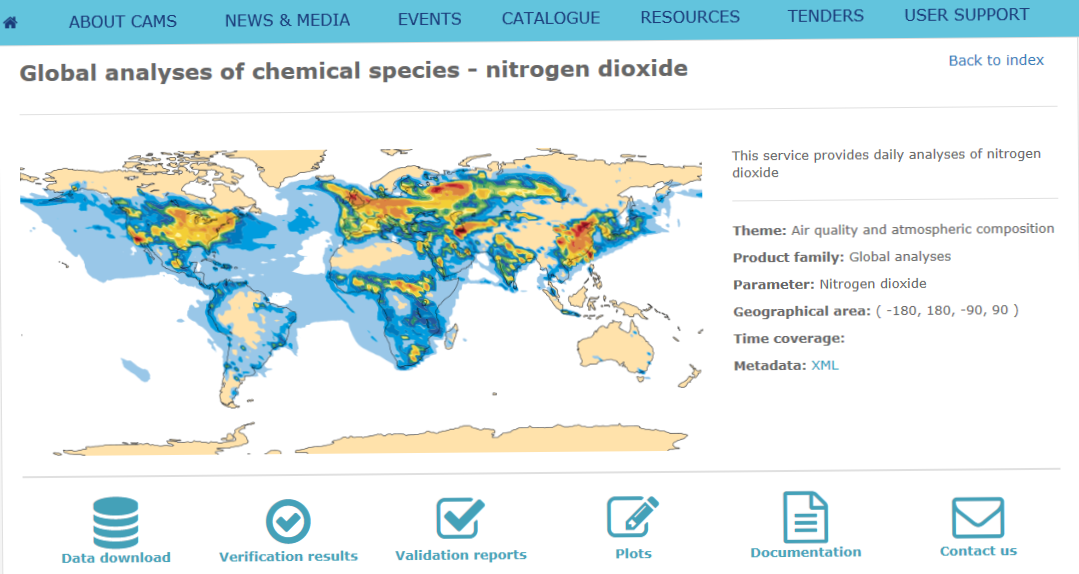
\includegraphics[keepaspectratio=true,width=\dimmin{}{\dimwidth{0.90}}]{images/catalogue}{}\mdline{599}%mdk

%mdk-data-line={600}
\mdhr{}%mdk

%mdk-data-line={601}
\noindent\mdline{601}\mdcaption{\textbf{Figure~\mdcaptionlabel{1}.}~\mdcaptiontext{Available options and details of CAMS Catalogue product ~\emph{Global analyses of chemical species - nitrogen dioxide}}}%mdk
%mdk
\end{mdcenter}\label{cams-catalogue}%mdk
%mdk
\end{figure}%mdk

%mdk-data-line={604}
\noindent\mdline{604}\textbf{For global products}\mdline{604}, \mdline{604}\emph{Plots}\mdline{604} links to a page within CAMS website where an interactive global map is provided.
Figure\mdline{605}~\mdref{global-map}{\mdcaptionlabel{2}}\mdline{605} shows the generated map of global analysis of NO\mdline{605}\mdsub{2}\mdline{605} concentration for 00:00 UTC December 4th, 2016.
Information about pollutant concentration is color-layered on the map with a measurement unit legend provided.
The user is able to adjust the date/time and the vertical area of interest.%mdk

%mdk-data-line={609}
\begin{figure}[h!]%mdk
\begin{mdcenter}%mdk

%mdk-data-line={610}
\noindent\mdline{610}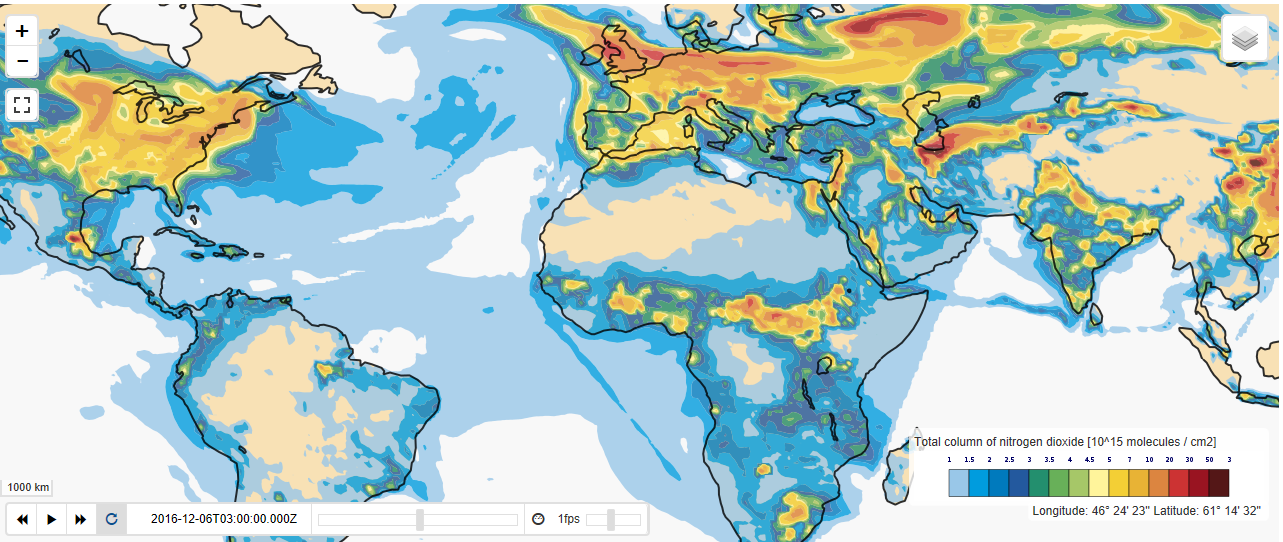
\includegraphics[keepaspectratio=true,width=\dimmin{}{\dimwidth{0.90}}]{images/global_map}{}\mdline{610}%mdk

%mdk-data-line={611}
\mdhr{}%mdk

%mdk-data-line={612}
\noindent\mdline{612}\mdcaption{\textbf{Figure~\mdcaptionlabel{2}.}~\mdcaptiontext{Global analysis of NO\mdsub{2} concentration for December 4th, 2016}}%mdk
%mdk
\end{mdcenter}\label{global-map}%mdk
%mdk
\end{figure}%mdk

%mdk-data-line={614}
\noindent\mdline{614}It should be noted that the plots service seems confusing at first, since both global analyses and forecasts link to the same page.
The distinction between analysis and forecast is based on the date/time selected in respect to current date/time.
Also, the plot service is time-limited in the sense that provides analyses for the past \mdline{616}$5$\mdline{616} days and forecasts for the following \mdline{616}$5$\mdline{616} days only.%mdk

%mdk-data-line={618}
\mdline{618}Global product \mdline{618}\emph{Data download}\mdline{618} link to a page within CAMS website where the user can choose to download data through an interactive interface or through ftp access.
Interactive data access link to ECMWF website. The user is presented a rich web form to select the exact product of interest. This is shown in Figure\mdline{619}~\mdref{global-data}{\mdcaptionlabel{3}}\mdline{619}.
A date-span or specific months can be selected, different vertical levels (surface or pressure dependent or model dependent), multiple time-steps and a huge parameter list, which of course includes dust, O\mdline{620}\mdsub{3}\mdline{620}, NO, NO\mdline{620}\mdsub{2}\mdline{620}.
A drawback is that data for the past four days in respect to current date is not available.%mdk

%mdk-data-line={623}
\begin{figure}[h!]%mdk
\begin{mdcenter}%mdk

%mdk-data-line={624}
\noindent\mdline{624}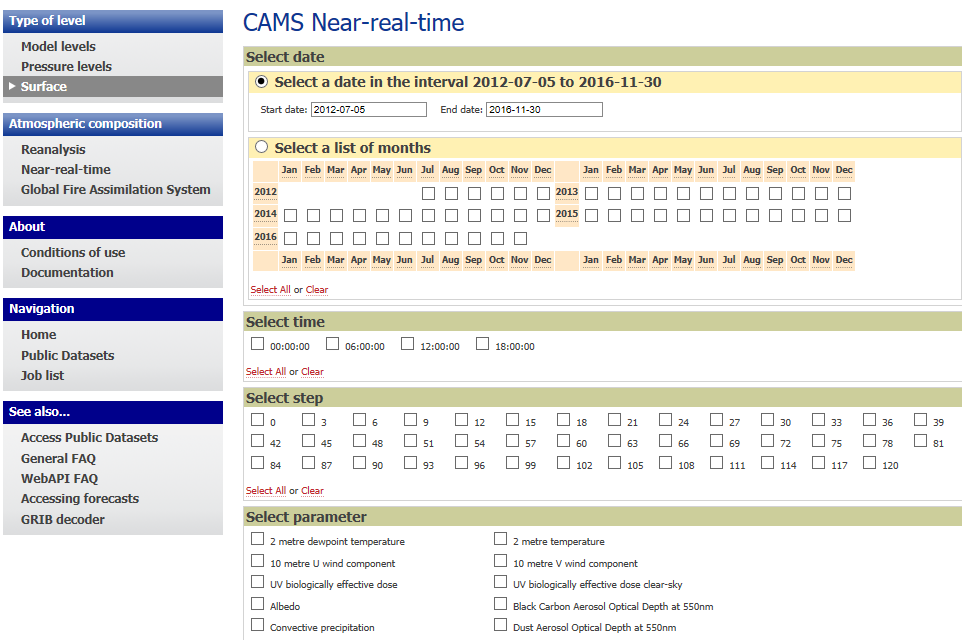
\includegraphics[keepaspectratio=true,width=\dimmin{}{\dimwidth{0.90}}]{images/global_real_time}{}\mdline{624}%mdk

%mdk-data-line={625}
\mdhr{}%mdk

%mdk-data-line={626}
\noindent\mdline{626}\mdcaption{\textbf{Figure~\mdcaptionlabel{3}.}~\mdcaptiontext{User Interface of ECMWF website for downloading data of global analyses and forecasts.}}%mdk
%mdk
\end{mdcenter}\label{global-data}%mdk
%mdk
\end{figure}%mdk

%mdk-data-line={628}
\noindent\mdline{628}After the user has set the filters he is able to download data in both GRID and NetCDF format by clicking the relative link.
In both cases he is led to an \mdline{629}\emph{Additional filtering}\mdline{629} form where he can define the area of interest and the grid resolution as shown in Figure\mdline{629}~\mdref{global-data-additional}{\mdcaptionlabel{4}}\mdline{629}.
The data is then available for downloading.%mdk

%mdk-data-line={632}
\begin{figure}[h!]%mdk
\begin{mdcenter}%mdk

%mdk-data-line={633}
\noindent\mdline{633}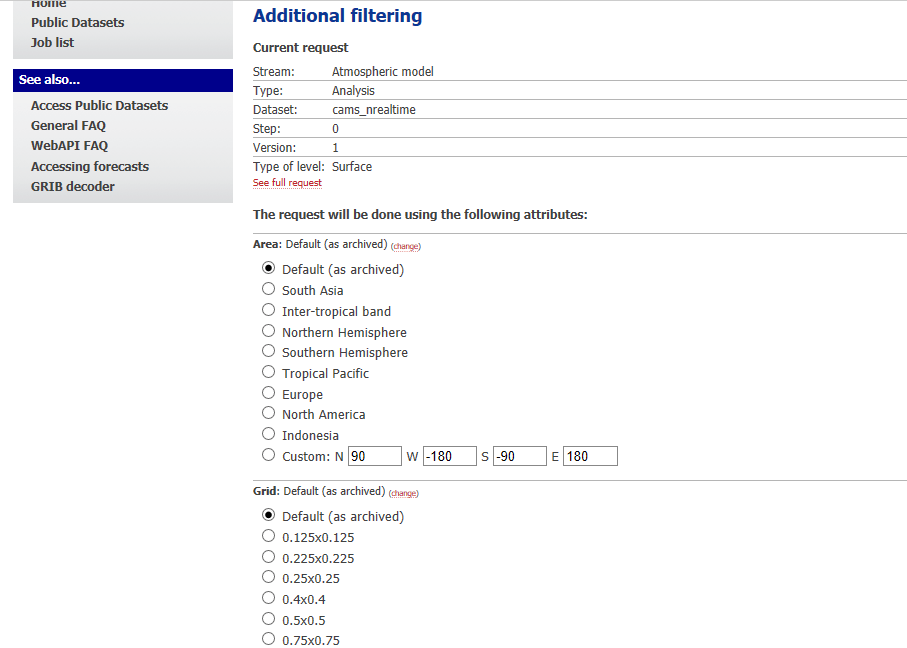
\includegraphics[keepaspectratio=true,width=\dimmin{}{\dimwidth{0.90}}]{images/global_real_time_additional}{}\mdline{633}%mdk

%mdk-data-line={634}
\mdhr{}%mdk

%mdk-data-line={635}
\noindent\mdline{635}\mdcaption{\textbf{Figure~\mdcaptionlabel{4}.}~\mdcaptiontext{Additional filtering of global analyses' and forecasts' data before downloading.}}%mdk
%mdk
\end{mdcenter}\label{global-data-additional}%mdk
%mdk
\end{figure}%mdk

%mdk-data-line={638}
\noindent\mdline{638}\textbf{For regional products}\mdline{638}, both \mdline{638}\emph{Plots}\mdline{638} and \mdline{638}\emph{Data download}\mdline{638} link to the regional subdomain of CAMS website.
The subdomain provides a universal access to individual models and ensemble plots and data for both analyses and forecasts.
This is done by an easy-to-use tab section as seen in Figure.%mdk

%mdk-data-line={642}
\mdline{642}In \mdline{642}\emph{Ensemble Analysis and Forecast}\mdline{642} tab, except from forecasts and analyses maps, additional plots of daily mean and maximum values as well as EPSgrams for 41 major European cities are available (Figure \mdline{642}\#\mdline{642}ensemble-tab).%mdk

%mdk-data-line={644}
\begin{figure}[h!]%mdk
\begin{mdcenter}%mdk

%mdk-data-line={645}
\noindent\mdline{645}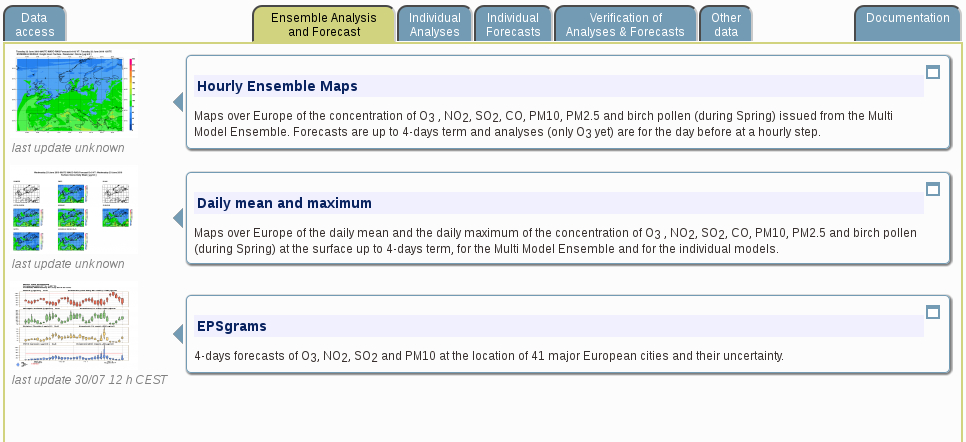
\includegraphics[keepaspectratio=true,width=\dimmin{}{\dimwidth{0.90}}]{images/ensemble_tab}{}\mdline{645}%mdk

%mdk-data-line={646}
\mdhr{}%mdk

%mdk-data-line={647}
\noindent\mdline{647}\mdcaption{\textbf{Figure~\mdcaptionlabel{5}.}~\mdcaptiontext{Available options in \emph{Ensemble Analysis and Forecast} tab}}%mdk
%mdk
\end{mdcenter}\label{ensemble-tab}%mdk
%mdk
\end{figure}%mdk

%mdk-data-line={649}
\noindent\mdline{649}\emph{Hourly Ensemble Maps}\mdline{649} (as well as all maps) provide a friendly user interface (UI) with details of the product, a time navigation bar, filters for base date/time, model, vertical level and parameter options.
The outline is shown in Figure\mdline{650}~\mdref{regional-map-details}{\mdcaptionlabel{6}}\mdline{650}.
\mdline{651}\emph{Hourly Ensemble Maps}\mdline{651} provide analysis and forecasts in the same UI. User first select a base date/time and then, depending on navigation\mdline{651}'\mdline{651}s bar value, he selects forecast or analysis produced on that day.
For example, if selected date/time is 00:00 UTC December 4th, 2016 and time navigation bar value is \mdline{652}$-10$\mdline{652}, then the analysis for 14:00 UTC December 3rd is depicted on the map.
Similarly, given the same date/time and a value of \mdline{653}$+48$\mdline{653} in time navigation bar, the forecast of 00:00 UTC December 6th is shown.
A useful \mdline{654}\emph{Download PDF}\mdline{654} button, which exports the map to PDF format, is also present.%mdk

%mdk-data-line={656}
\mdline{656}In order to obtain the analysis on 00:00 UTC December 4th, 2016 we set as date/time the December 5th and a time step of \mdline{656}$-24$\mdline{656}.
A sample obtained map is shown in Figure\mdline{657}~\mdref{ensemble-maps}{\mdcaptionlabel{7}}\mdline{657}.%mdk

%mdk-data-line={659}
\begin{figure}[h!]%mdk
\begin{mdcenter}%mdk

%mdk-data-line={660}
\noindent\mdline{660}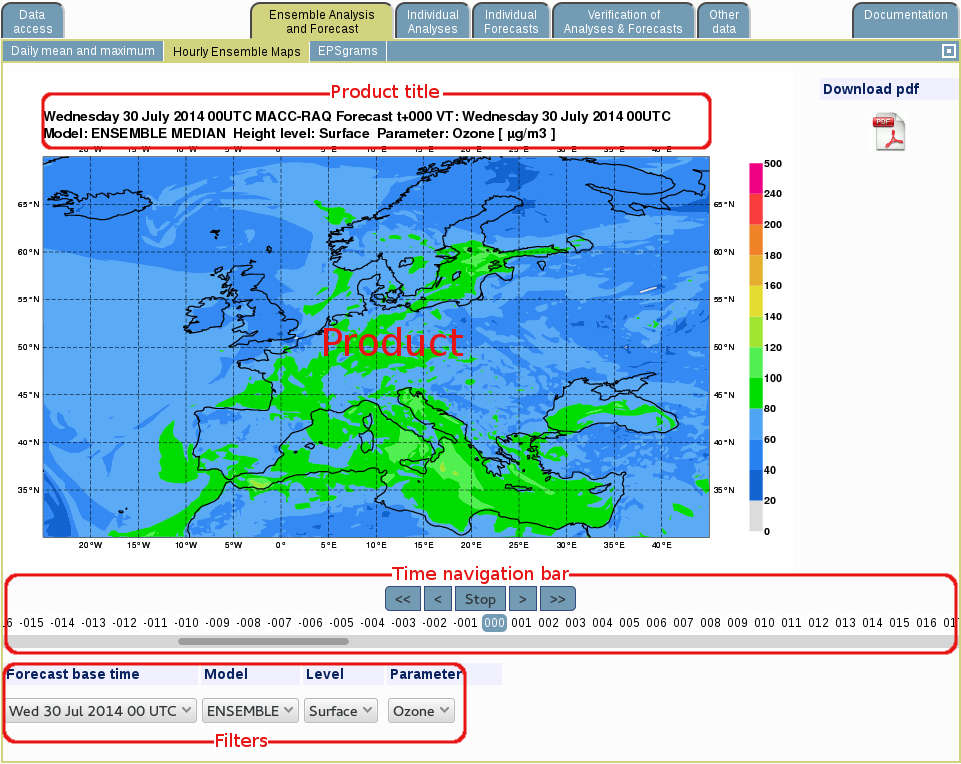
\includegraphics[keepaspectratio=true,width=\dimmin{}{\dimwidth{0.90}}]{images/regional_map_details}{}\mdline{660}%mdk

%mdk-data-line={661}
\mdhr{}%mdk

%mdk-data-line={662}
\noindent\mdline{662}\mdcaption{\textbf{Figure~\mdcaptionlabel{6}.}~\mdcaptiontext{Outline of analyses and forecast maps of regional products.}}%mdk
%mdk
\end{mdcenter}\label{regional-map-details}%mdk
%mdk
\end{figure}%mdk

%mdk-data-line={664}
\begin{figure}[h!]%mdk
\begin{mdcenter}%mdk

%mdk-data-line={665}
\noindent\mdline{665}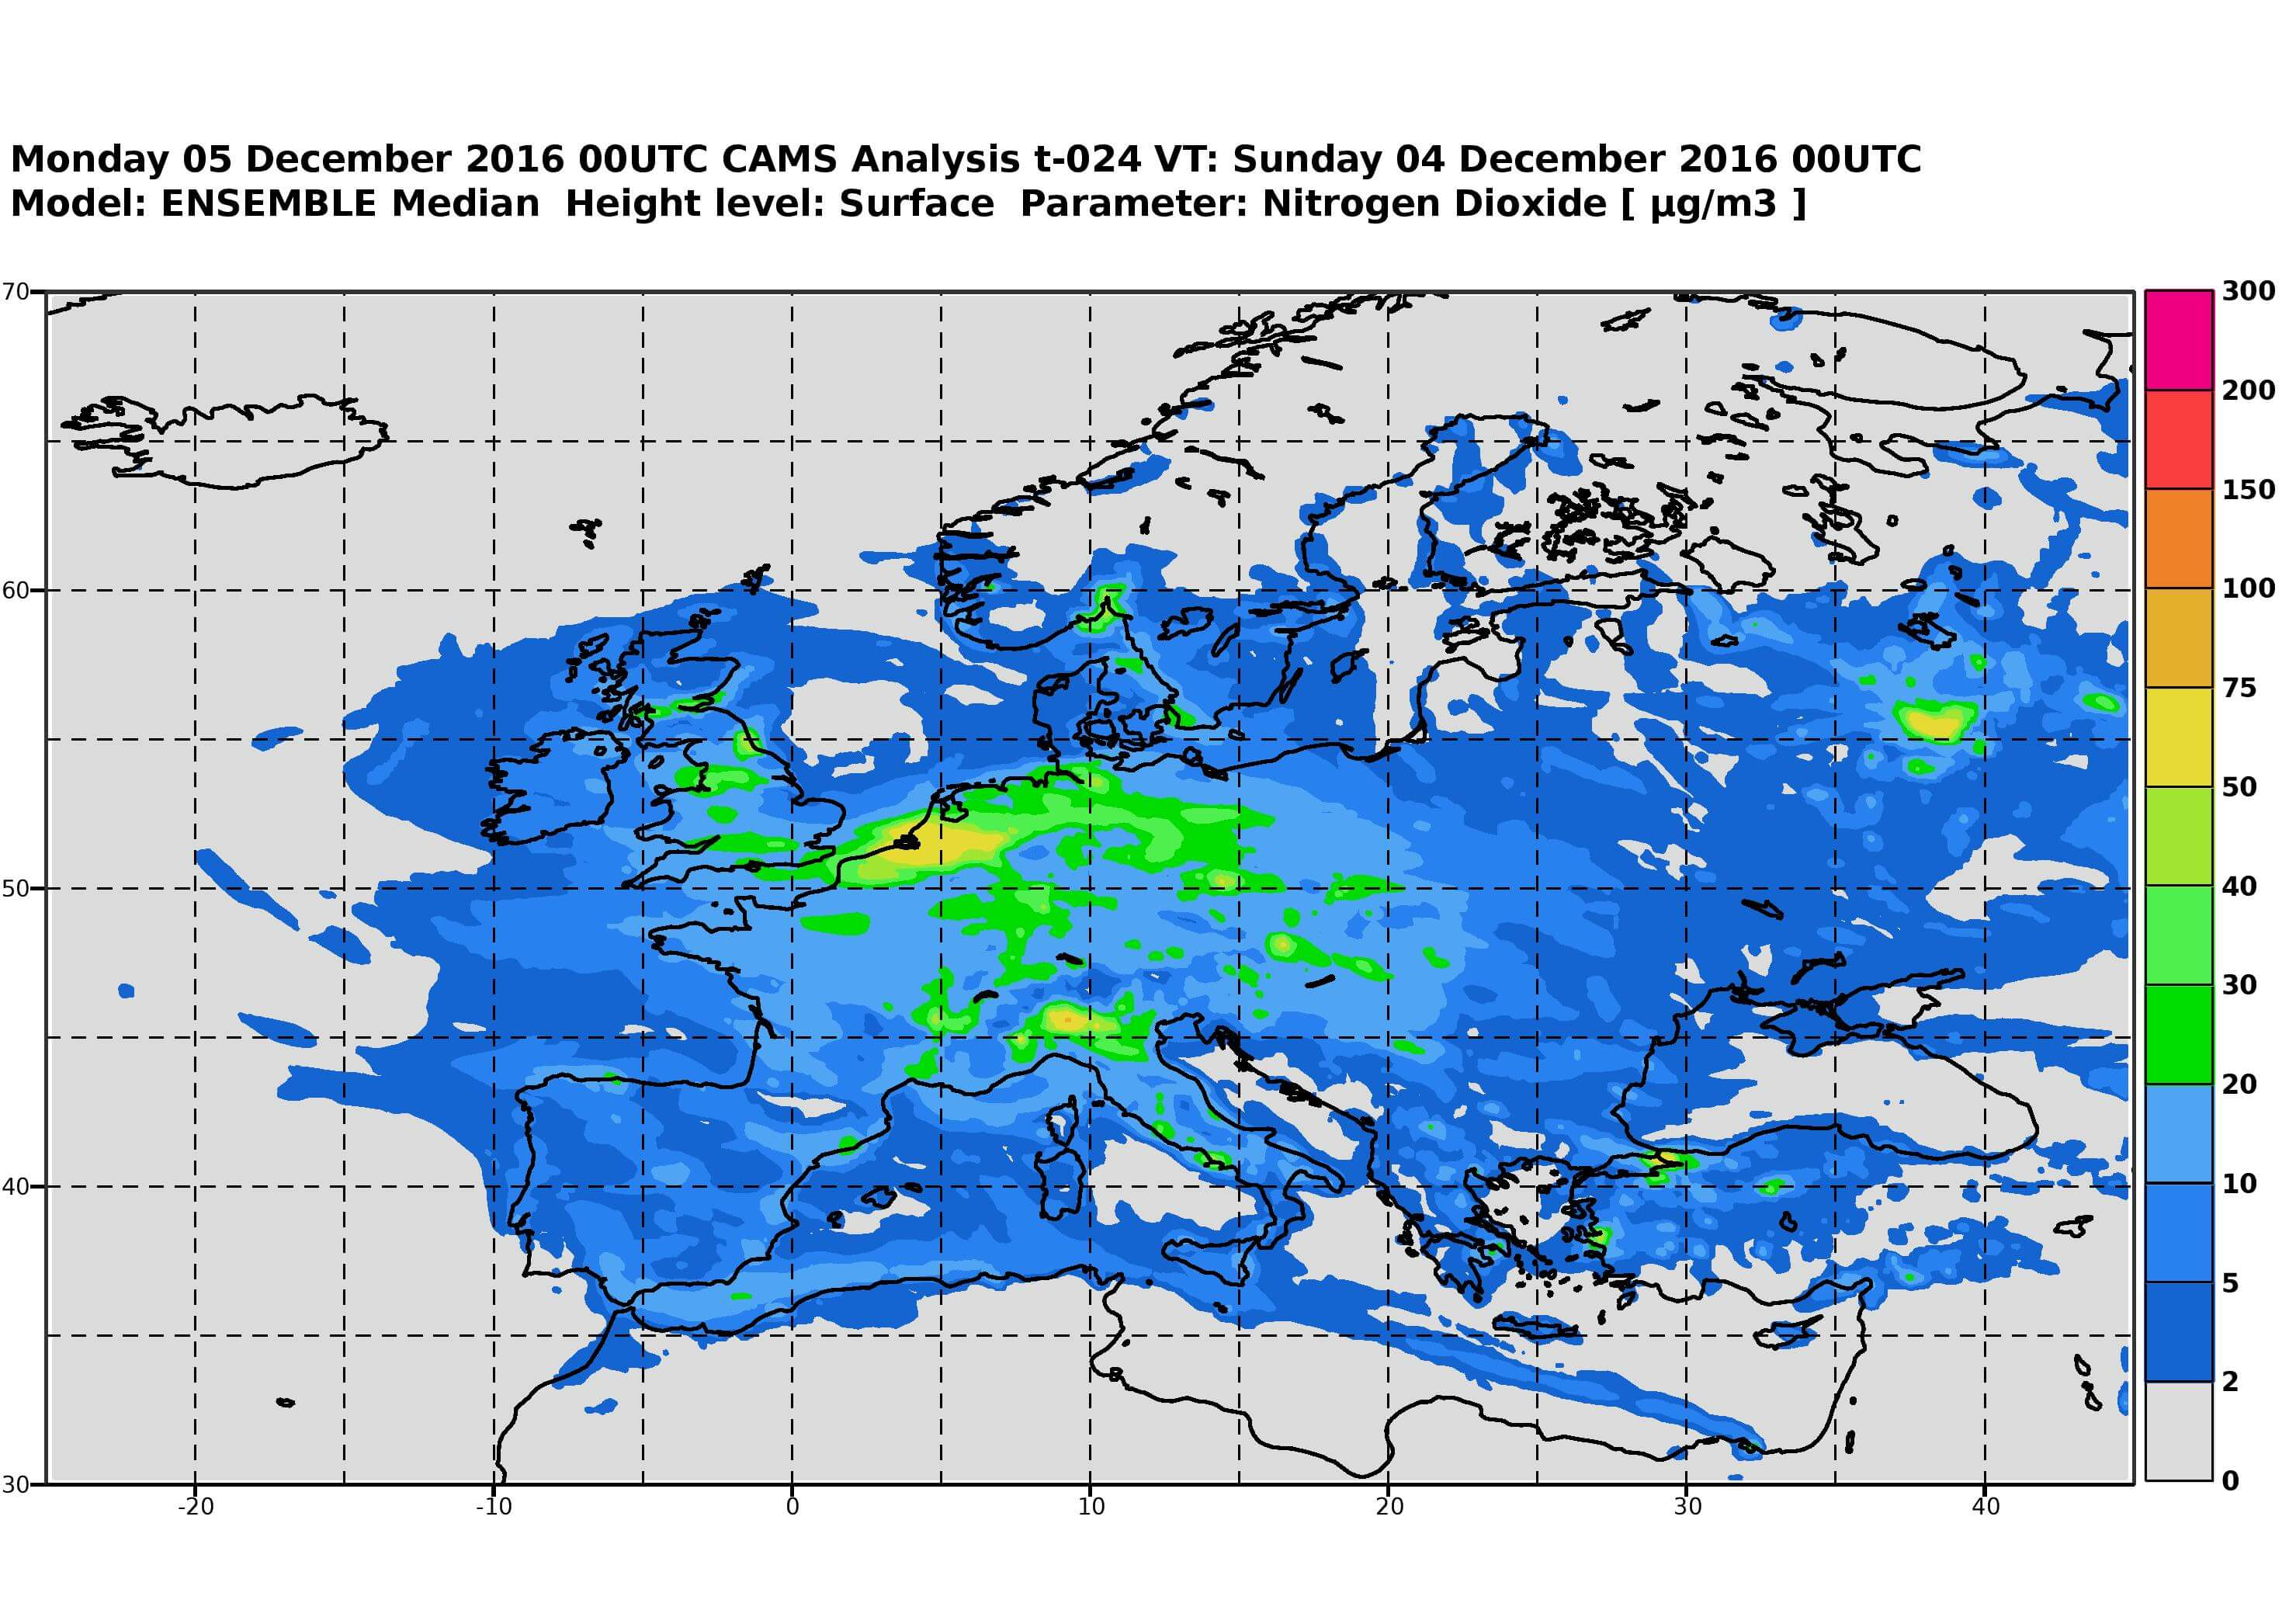
\includegraphics[keepaspectratio=true,width=\dimmin{}{\dimwidth{0.90}}]{images/ensemble_analysis_surface}{}\mdline{665}%mdk

%mdk-data-line={666}
\mdhr{}%mdk

%mdk-data-line={667}
\noindent\mdline{667}\mdcaption{\textbf{Figure~\mdcaptionlabel{7}.}~\mdcaptiontext{Analysis of NO\mdsub{2} concentration on 00:00 UTC December 4th, 2016 issued from the ENSEMBLE model.}}%mdk
%mdk
\end{mdcenter}\label{ensemble-maps}%mdk
%mdk
\end{figure}%mdk

%mdk-data-line={669}
\noindent\mdline{669}\emph{Daily mean and maximum}\mdline{669} tab provides maps of the daily mean and maximum values of the concentration of pollutants as calculated by each model and ensemble.
A useful feature is the ability to view the maps generated of all models side by side.
This feature is shown in Figure\mdline{671}~\mdref{regional-maximum}{\mdcaptionlabel{8}}\mdline{671} for NO\mdline{671}\mdsub{2}\mdline{671} maximum concentration values on December 4th, 2016.%mdk

%mdk-data-line={673}
\begin{figure}[h!]%mdk
\begin{mdcenter}%mdk

%mdk-data-line={674}
\noindent\mdline{674}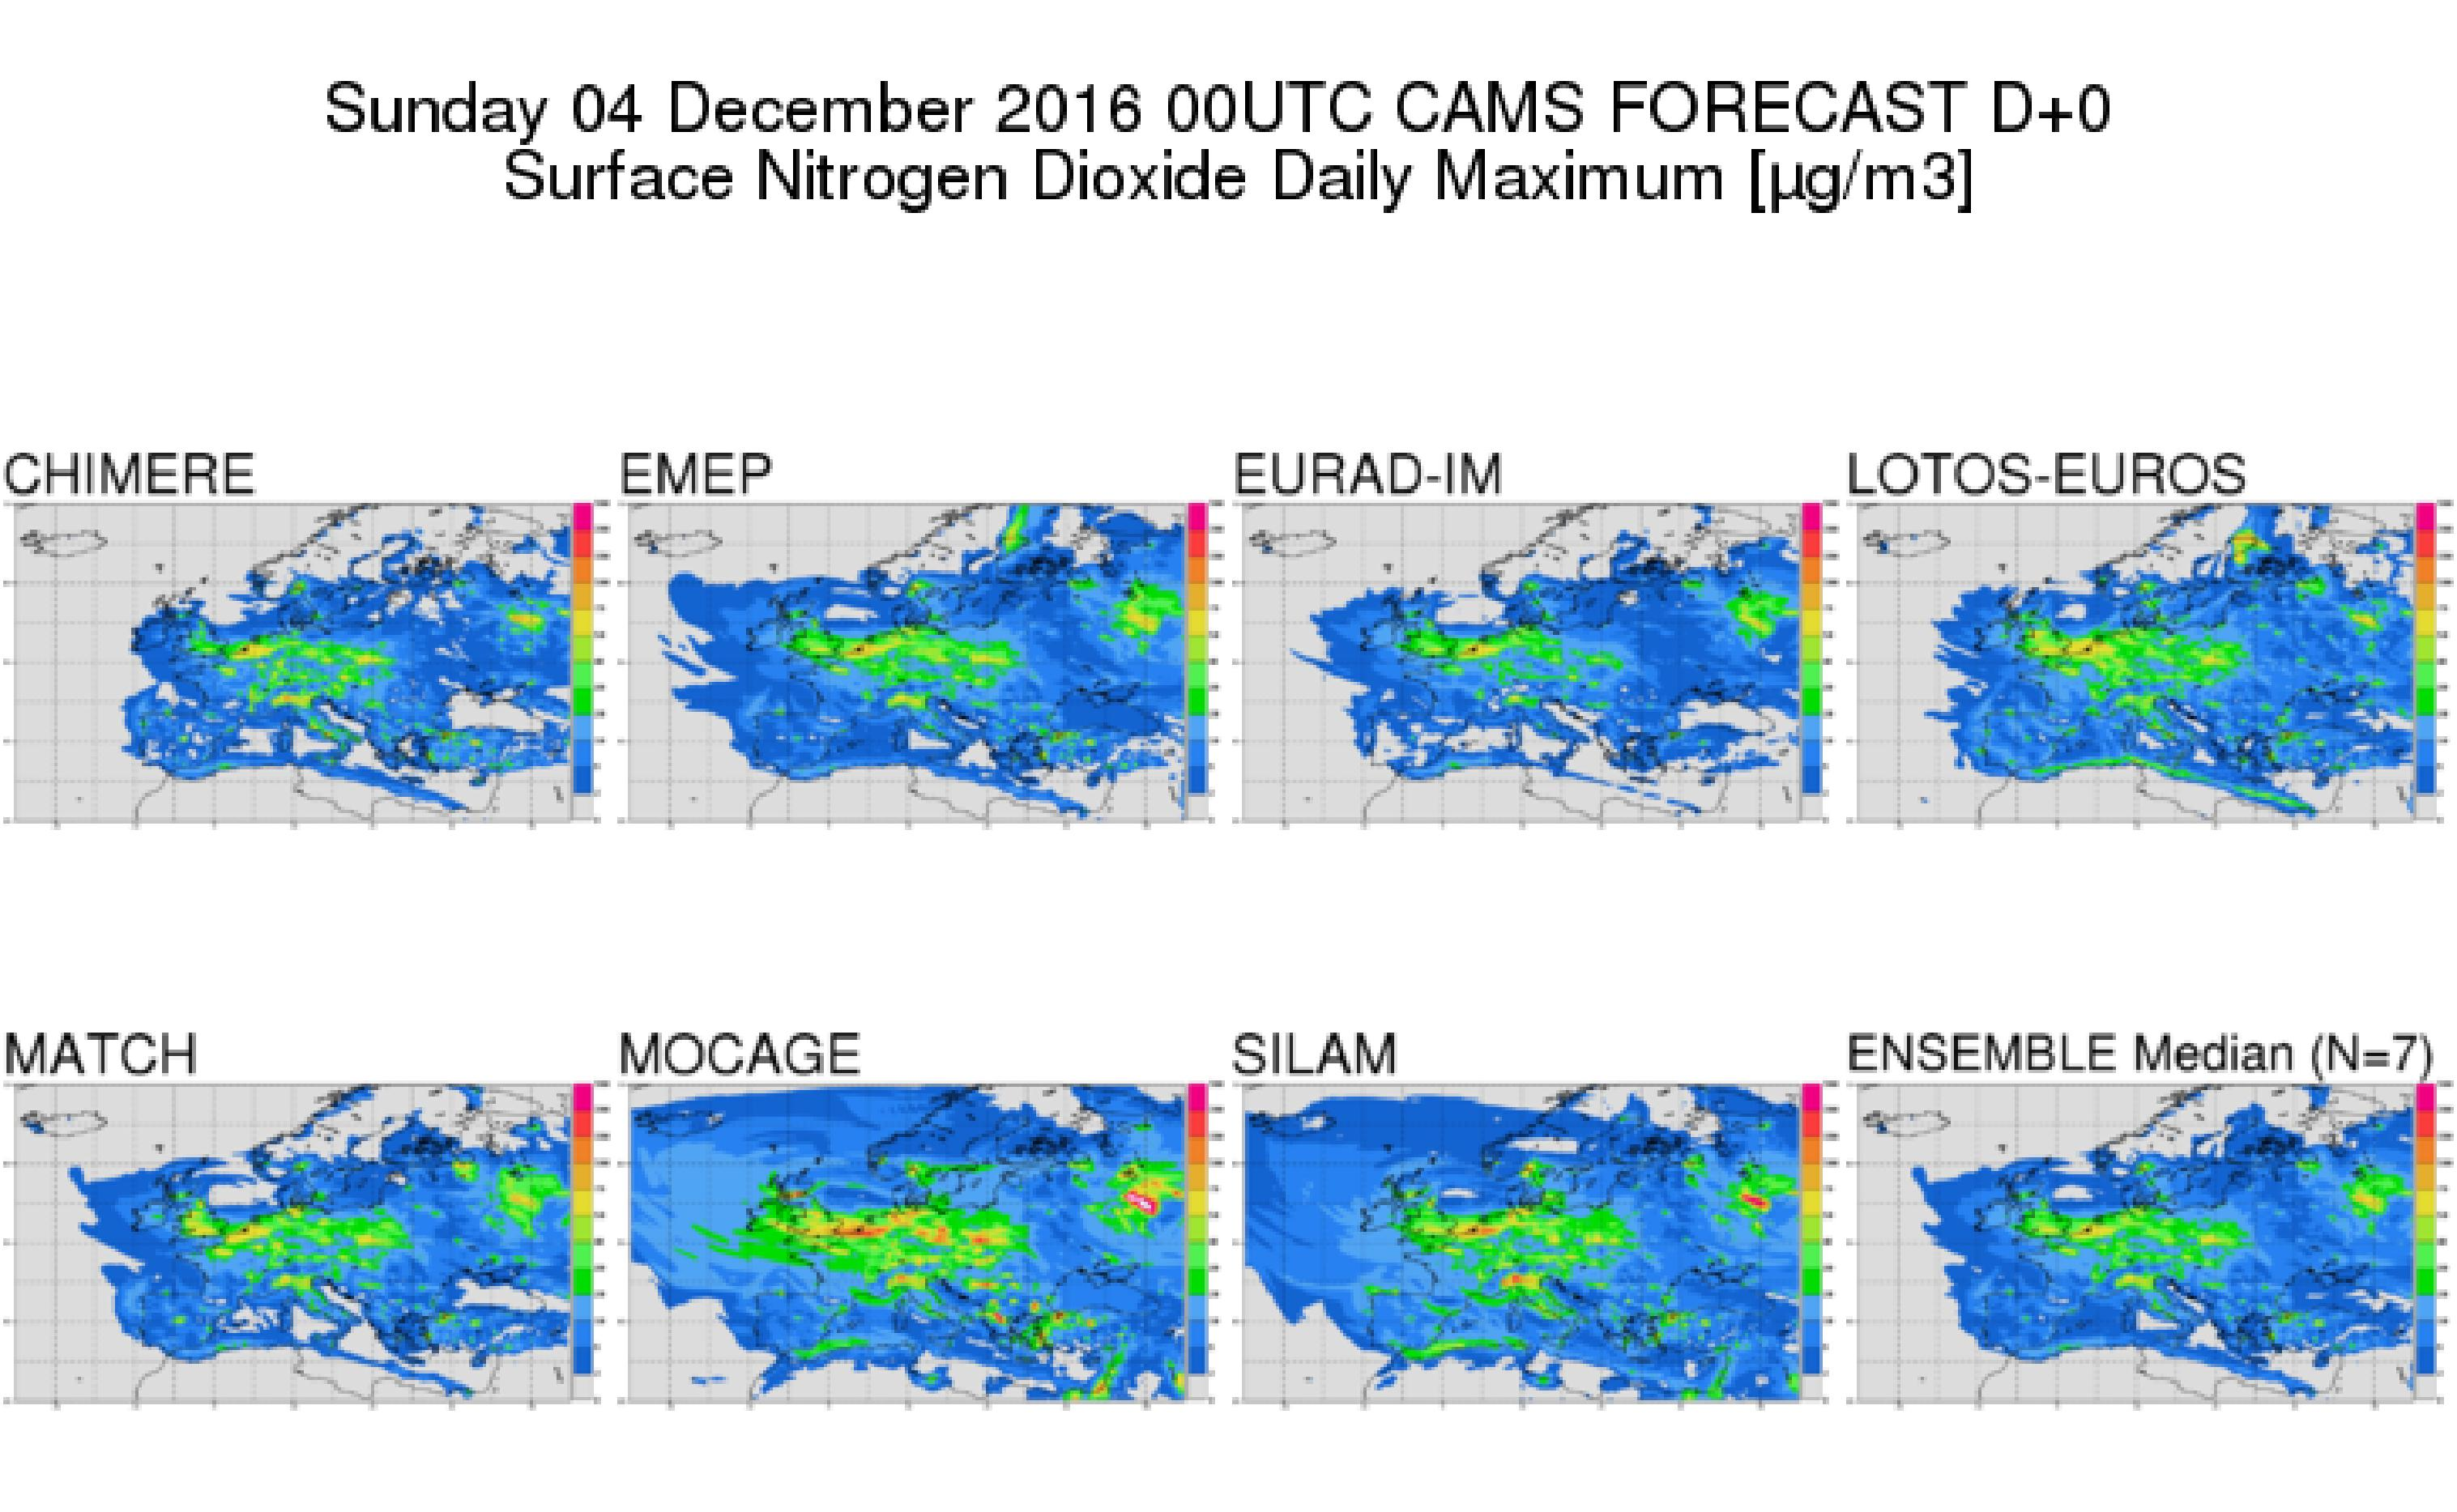
\includegraphics[keepaspectratio=true,width=\dimmin{}{\dimwidth{0.90}}]{images/regional_maximum}{}\mdline{674}%mdk

%mdk-data-line={675}
\mdhr{}%mdk

%mdk-data-line={676}
\noindent\mdline{676}\mdcaption{\textbf{Figure~\mdcaptionlabel{8}.}~\mdcaptiontext{Maximum concentrations of NO\mdsub{2} on December 4th, 2016 as calculated from all models and their ensemble.}}%mdk
%mdk
\end{mdcenter}\label{regional-maximum}%mdk
%mdk
\end{figure}%mdk

%mdk-data-line={678}
\noindent\mdline{678}\emph{EPSgrams}\mdline{678} tab provide 4-days forecasts of O\mdline{678}\mdsub{3}\mdline{678}, NO\mdline{678}\mdsub{2}\mdline{678}, SO\mdline{678}\mdsub{2}\mdline{678} and PM\mdline{678}\mdsub{10}\mdline{678} at the location of 41 major European cities and their uncertainty.
In Figure\mdline{679}~\mdref{regional-epsgram}{\mdcaptionlabel{9}}\mdline{679} forecasts for the city of Athens between December 4th and December 8th, 2016 are shown.%mdk

%mdk-data-line={681}
\begin{figure}[h!]%mdk
\begin{mdcenter}%mdk

%mdk-data-line={682}
\noindent\mdline{682}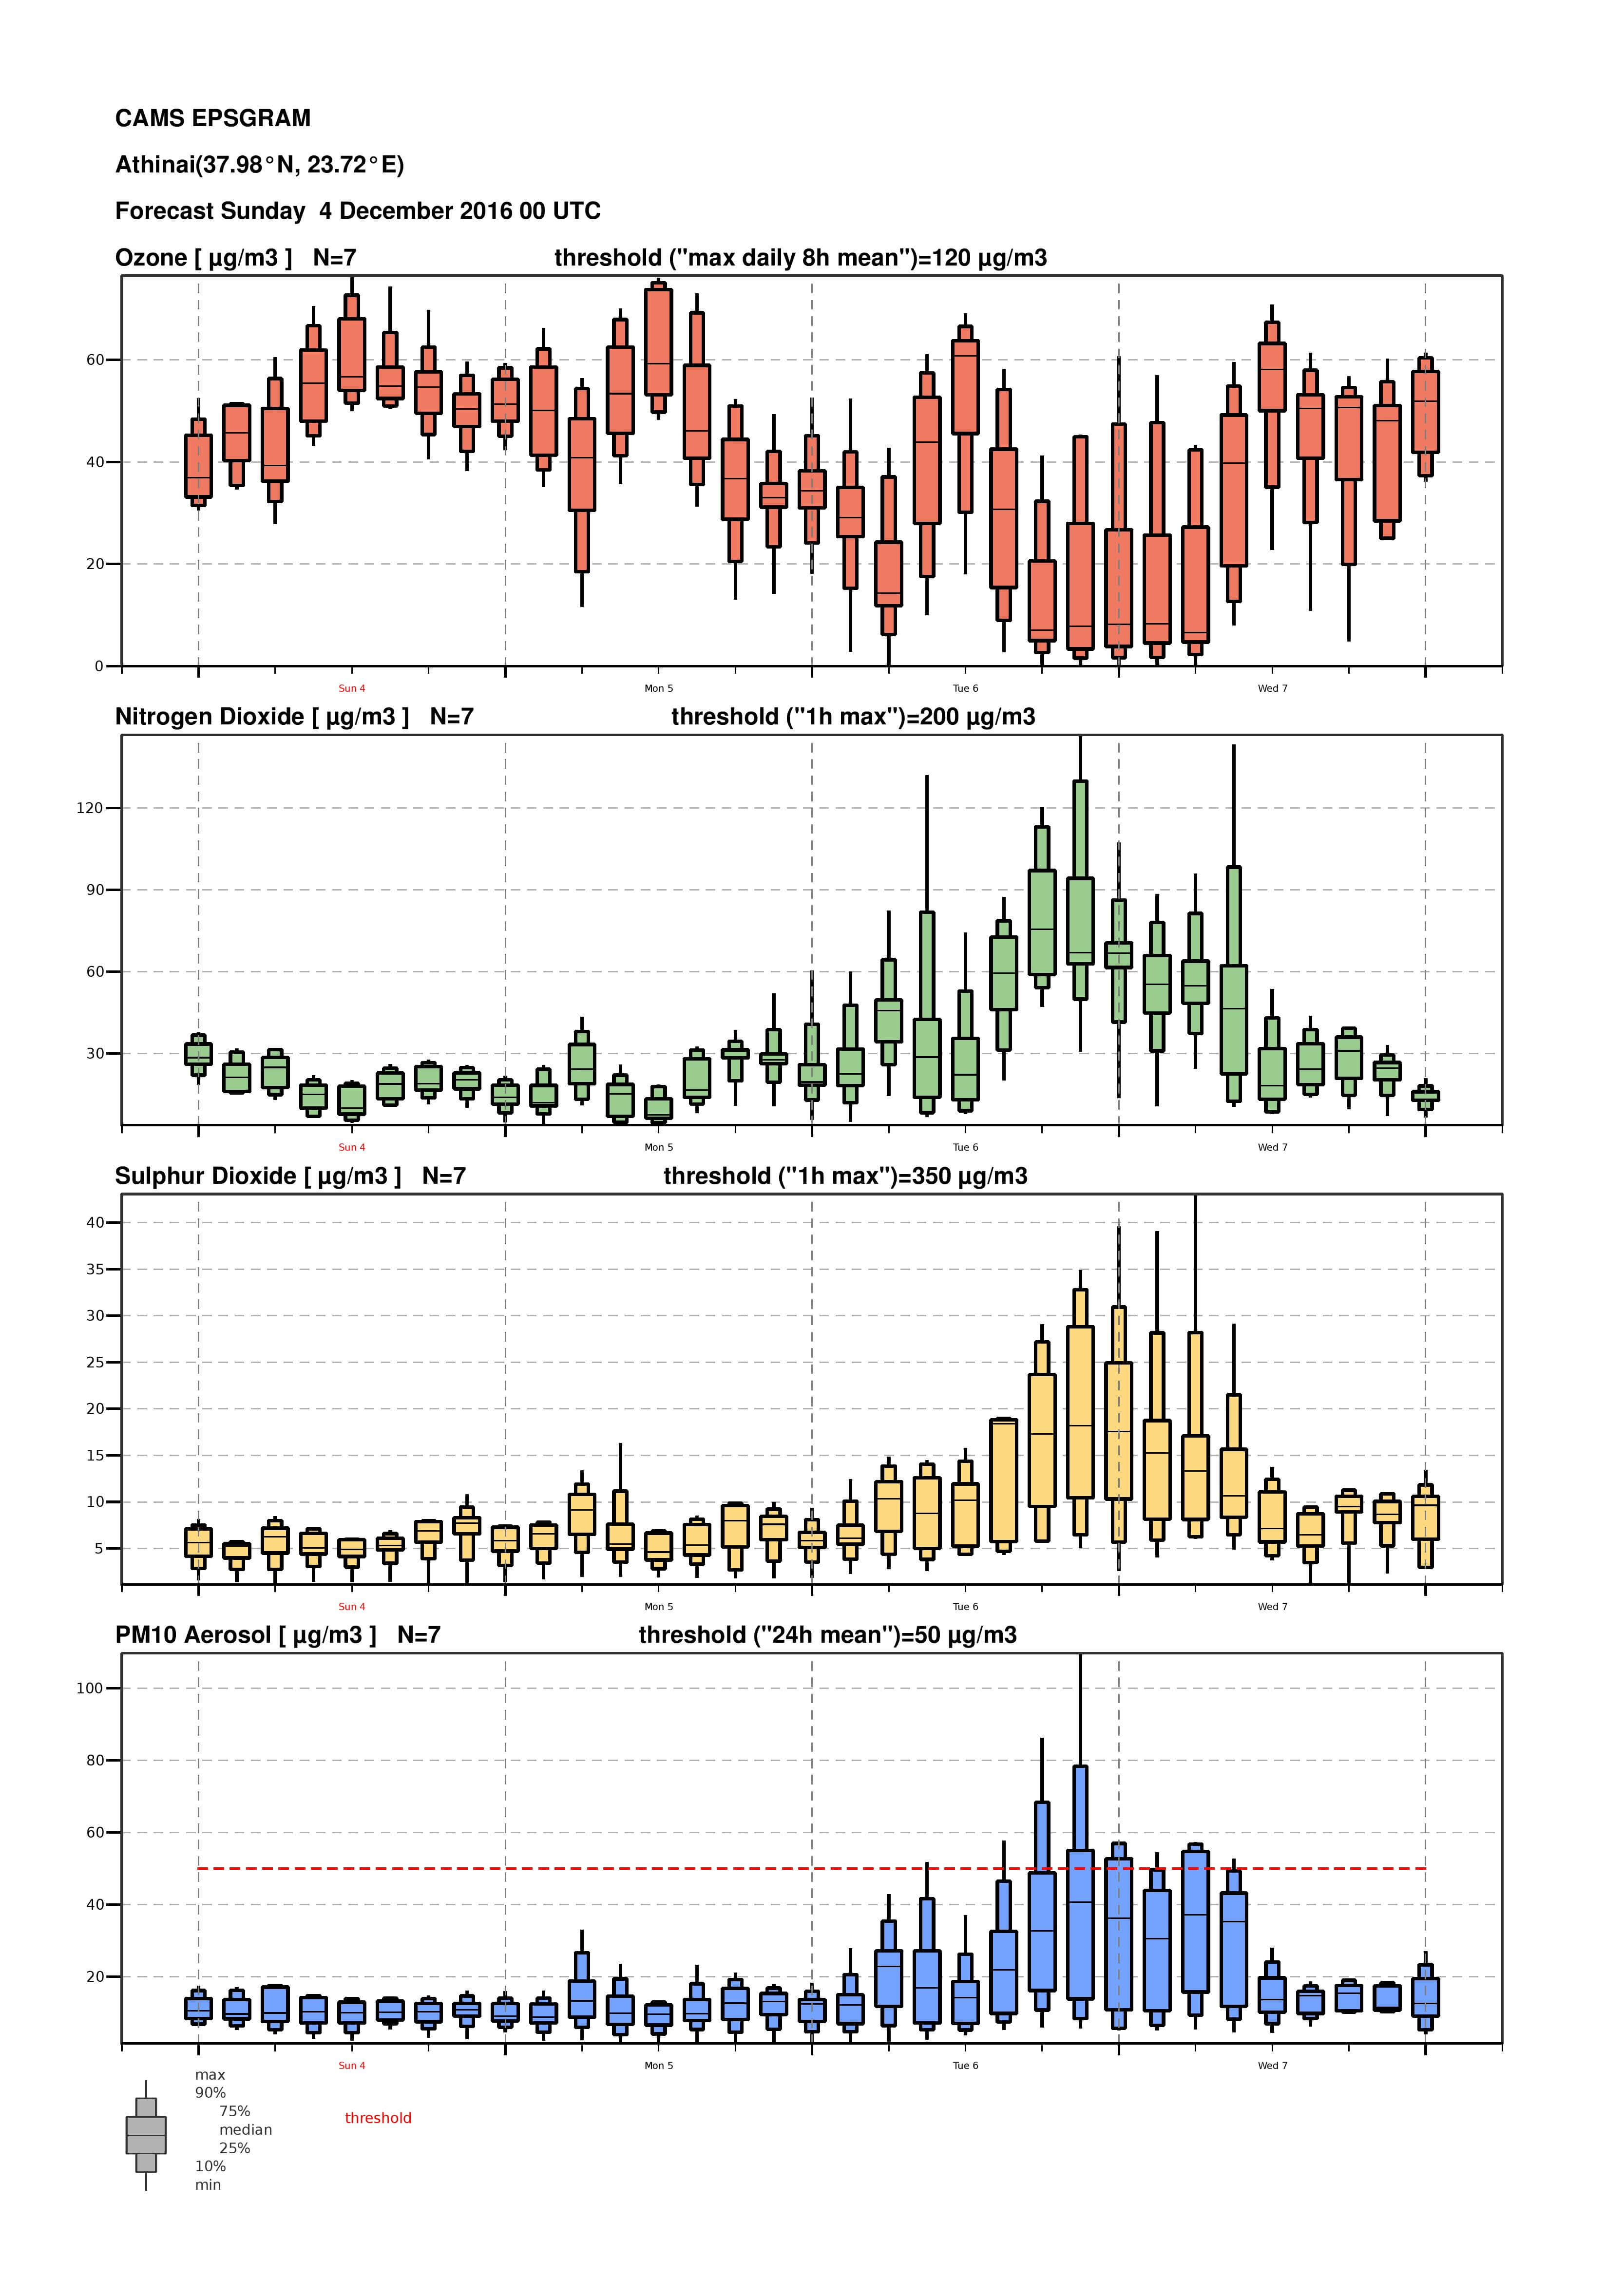
\includegraphics[keepaspectratio=true,width=\dimmin{}{\dimwidth{0.90}}]{images/regional-epsgram}{}\mdline{682}%mdk

%mdk-data-line={683}
\mdhr{}%mdk

%mdk-data-line={684}
\noindent\mdline{684}\mdcaption{\textbf{Figure~\mdcaptionlabel{9}.}~\mdcaptiontext{4-day forecast of O\mdsub{3}, NO\mdsub{2}, SO\mdsub{2} and PM\mdsub{10} at the city of Athens for the period between December 4th - December 8th, 2016.}}%mdk
%mdk
\end{mdcenter}\label{regional-epsgram}%mdk
%mdk
\end{figure}%mdk

%mdk-data-line={687}
\noindent\mdline{687}\emph{Individual Analyses}\mdline{687} and \mdline{687}\emph{Individual Forecasts}\mdline{687} tabs provide maps of pollutants\mdline{687}'\mdline{687} concentration based on individual models calculations.
Analyses are available for the day before at an hourly step.
Forecasts are available up to 4 days ahead at an hourly step.
It is interesting to see the relevance of the forecast for a given date/time to the post-analysis.
In Figure\mdline{691}~\mdref{chimere-map}{\mdcaptionlabel{10}}\mdline{691} we see the forecast of NO\mdline{691}\mdsub{2}\mdline{691} concentration for December 4th, 2016 issued on December 3rd and the relevant analysis issued on December 5th.
It is obvious that results are quite different.%mdk

%mdk-data-line={694}
\begin{figure}[h!]%mdk
\begin{mdcenter}%mdk
\mdinline{vertical-align=bottom,text-align=center}{\begin{mdtabular}{2}{\dimeval{(\linewidth)/2}}{0pt}%mdk
\begin{tabular}{cc}

%mdk-data-line={696}
\begin{mdcolumn}%mdk
\begin{mdblock}{padding=0.5ex,vertical-align=bottom,text-align=center,width=\dimavailable}%mdk
\mdline{697}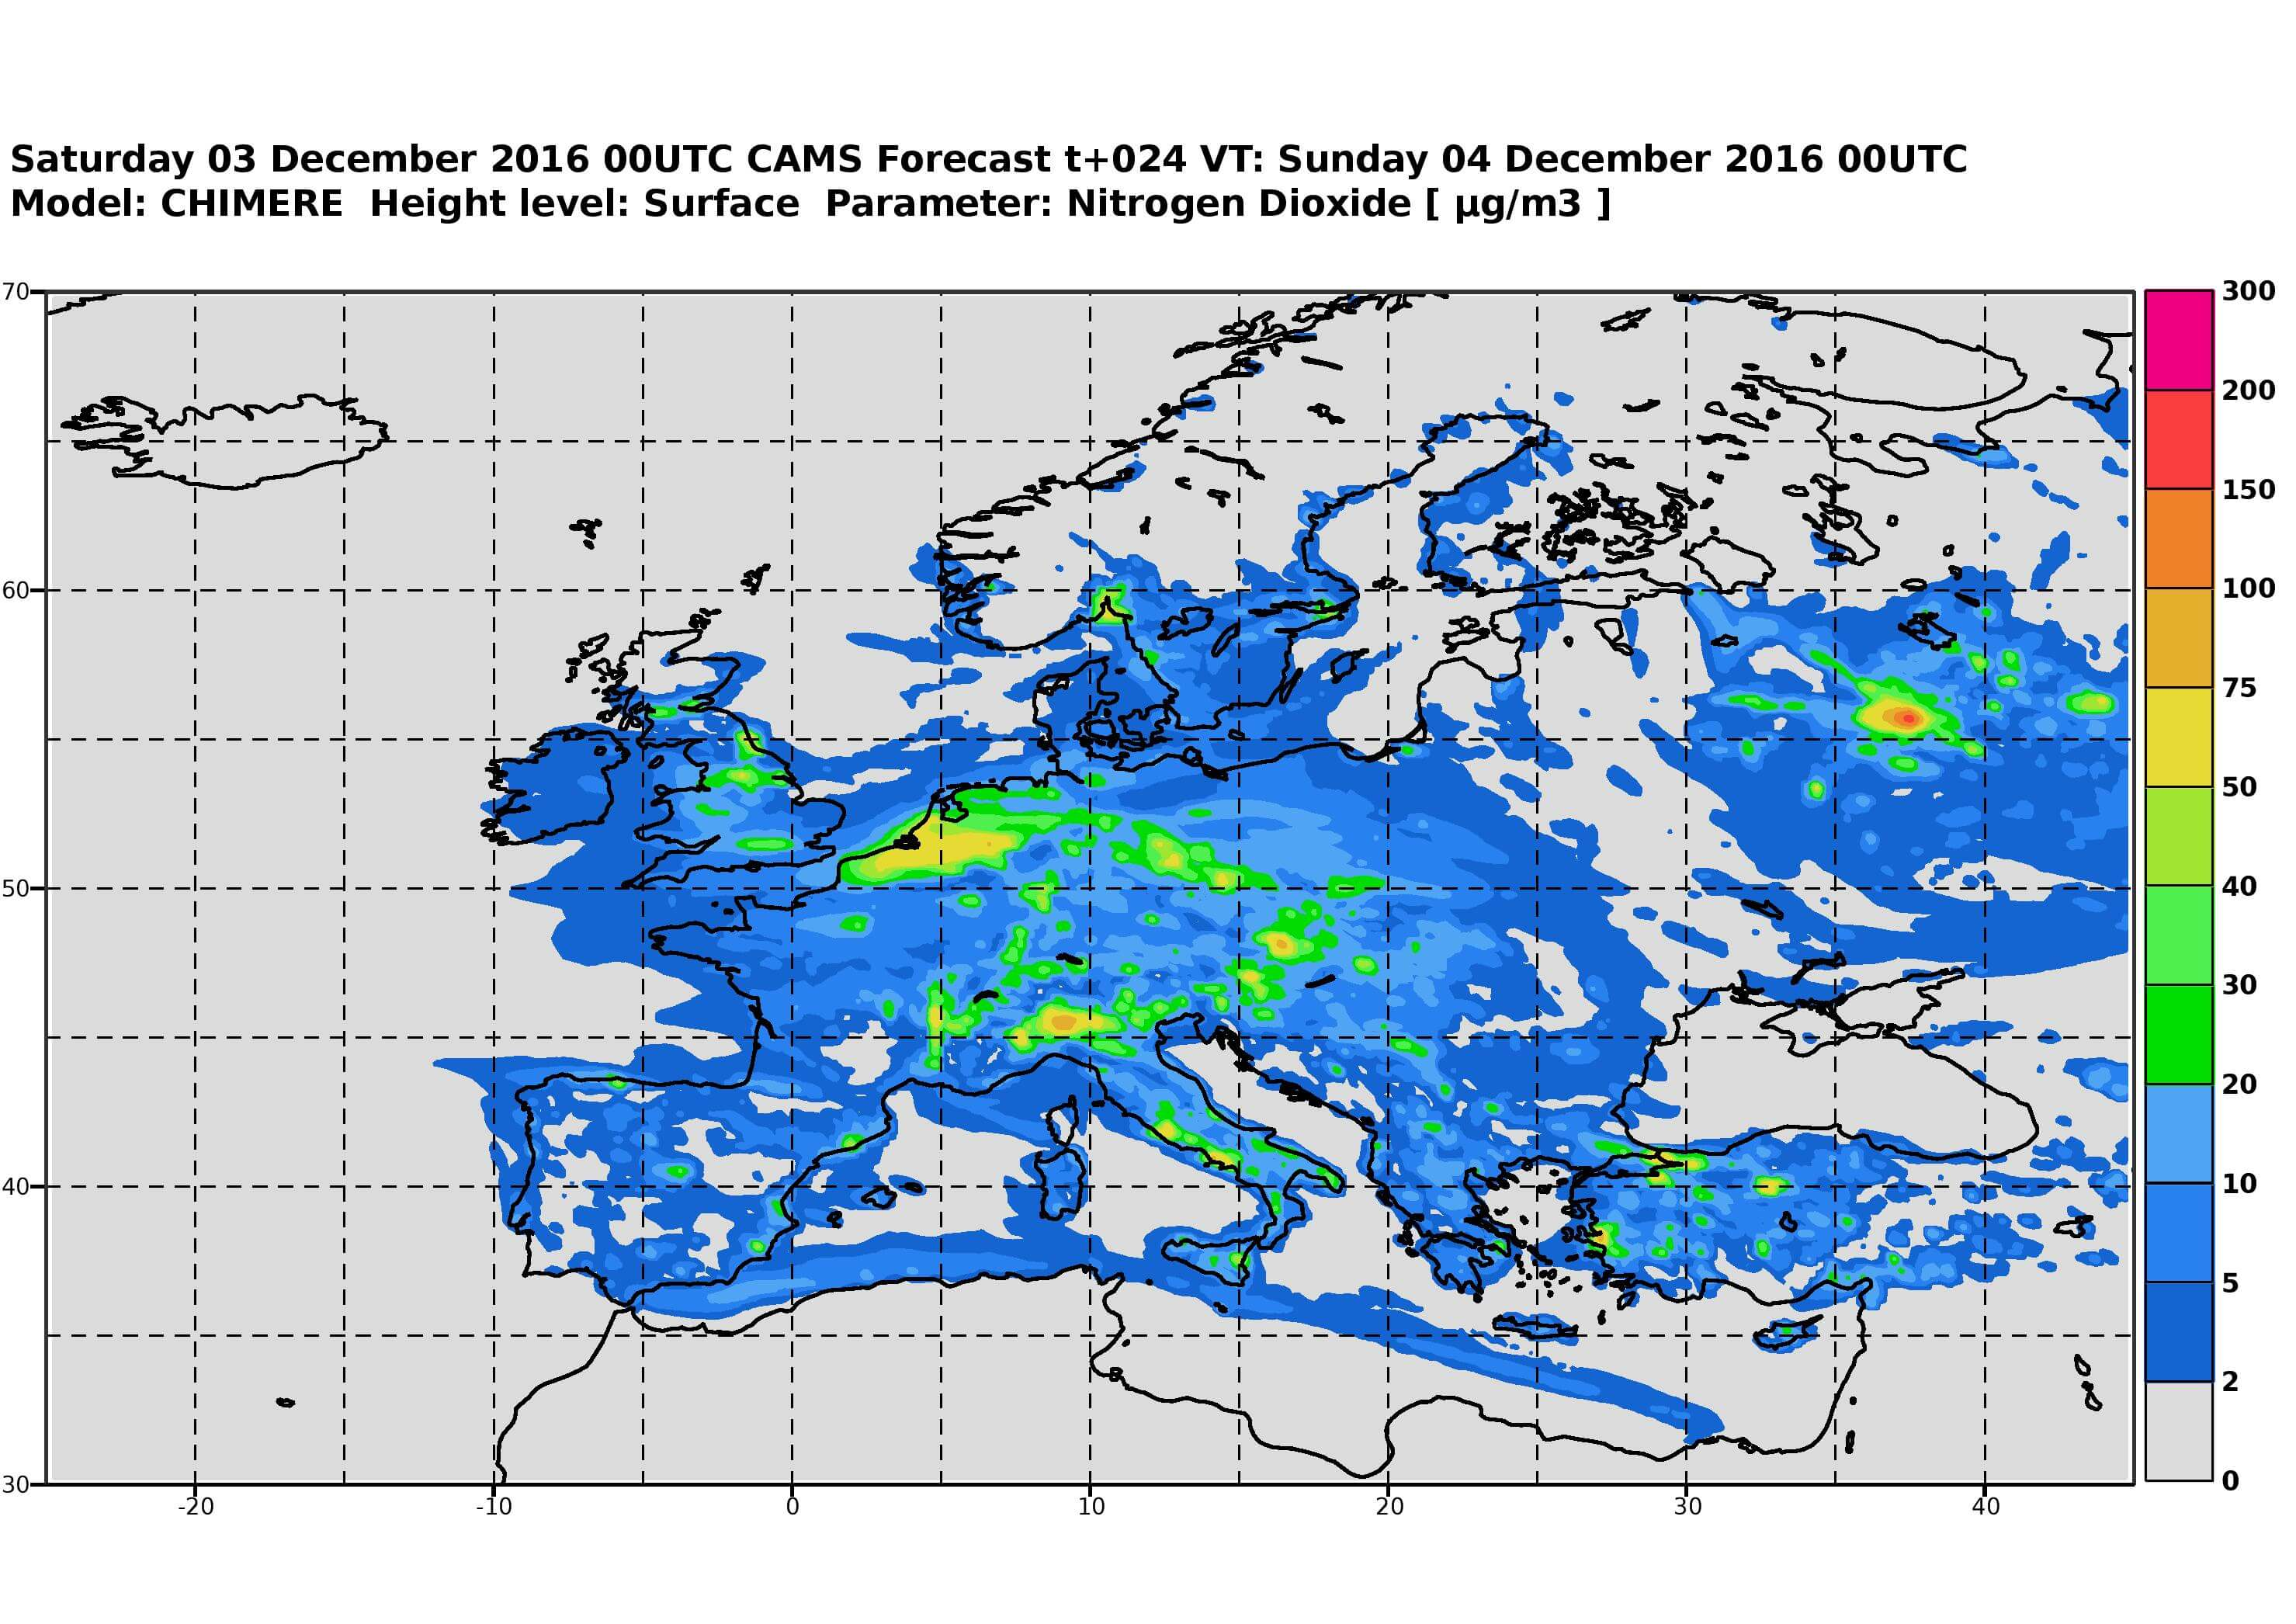
\includegraphics[keepaspectratio=true,width=\dimmin{}{\dimwidth{0.90}}]{images/chimere_forecast}{}\mdline{697}

%mdk-data-line={698}
\begin{mdbmargintb}{1ex}{}%mdk
\mdline{699}(a) \mdline{699} Forecast issued on December 3rd, 2016%mdk
\end{mdbmargintb}%mdk%mdk
\end{mdblock}%mdk
\end{mdcolumn}%mdk
&
%mdk-data-line={699}
\begin{mdcolumn}%mdk
\begin{mdblock}{padding=0.5ex,vertical-align=bottom,text-align=center,width=\dimavailable}%mdk
\mdline{700}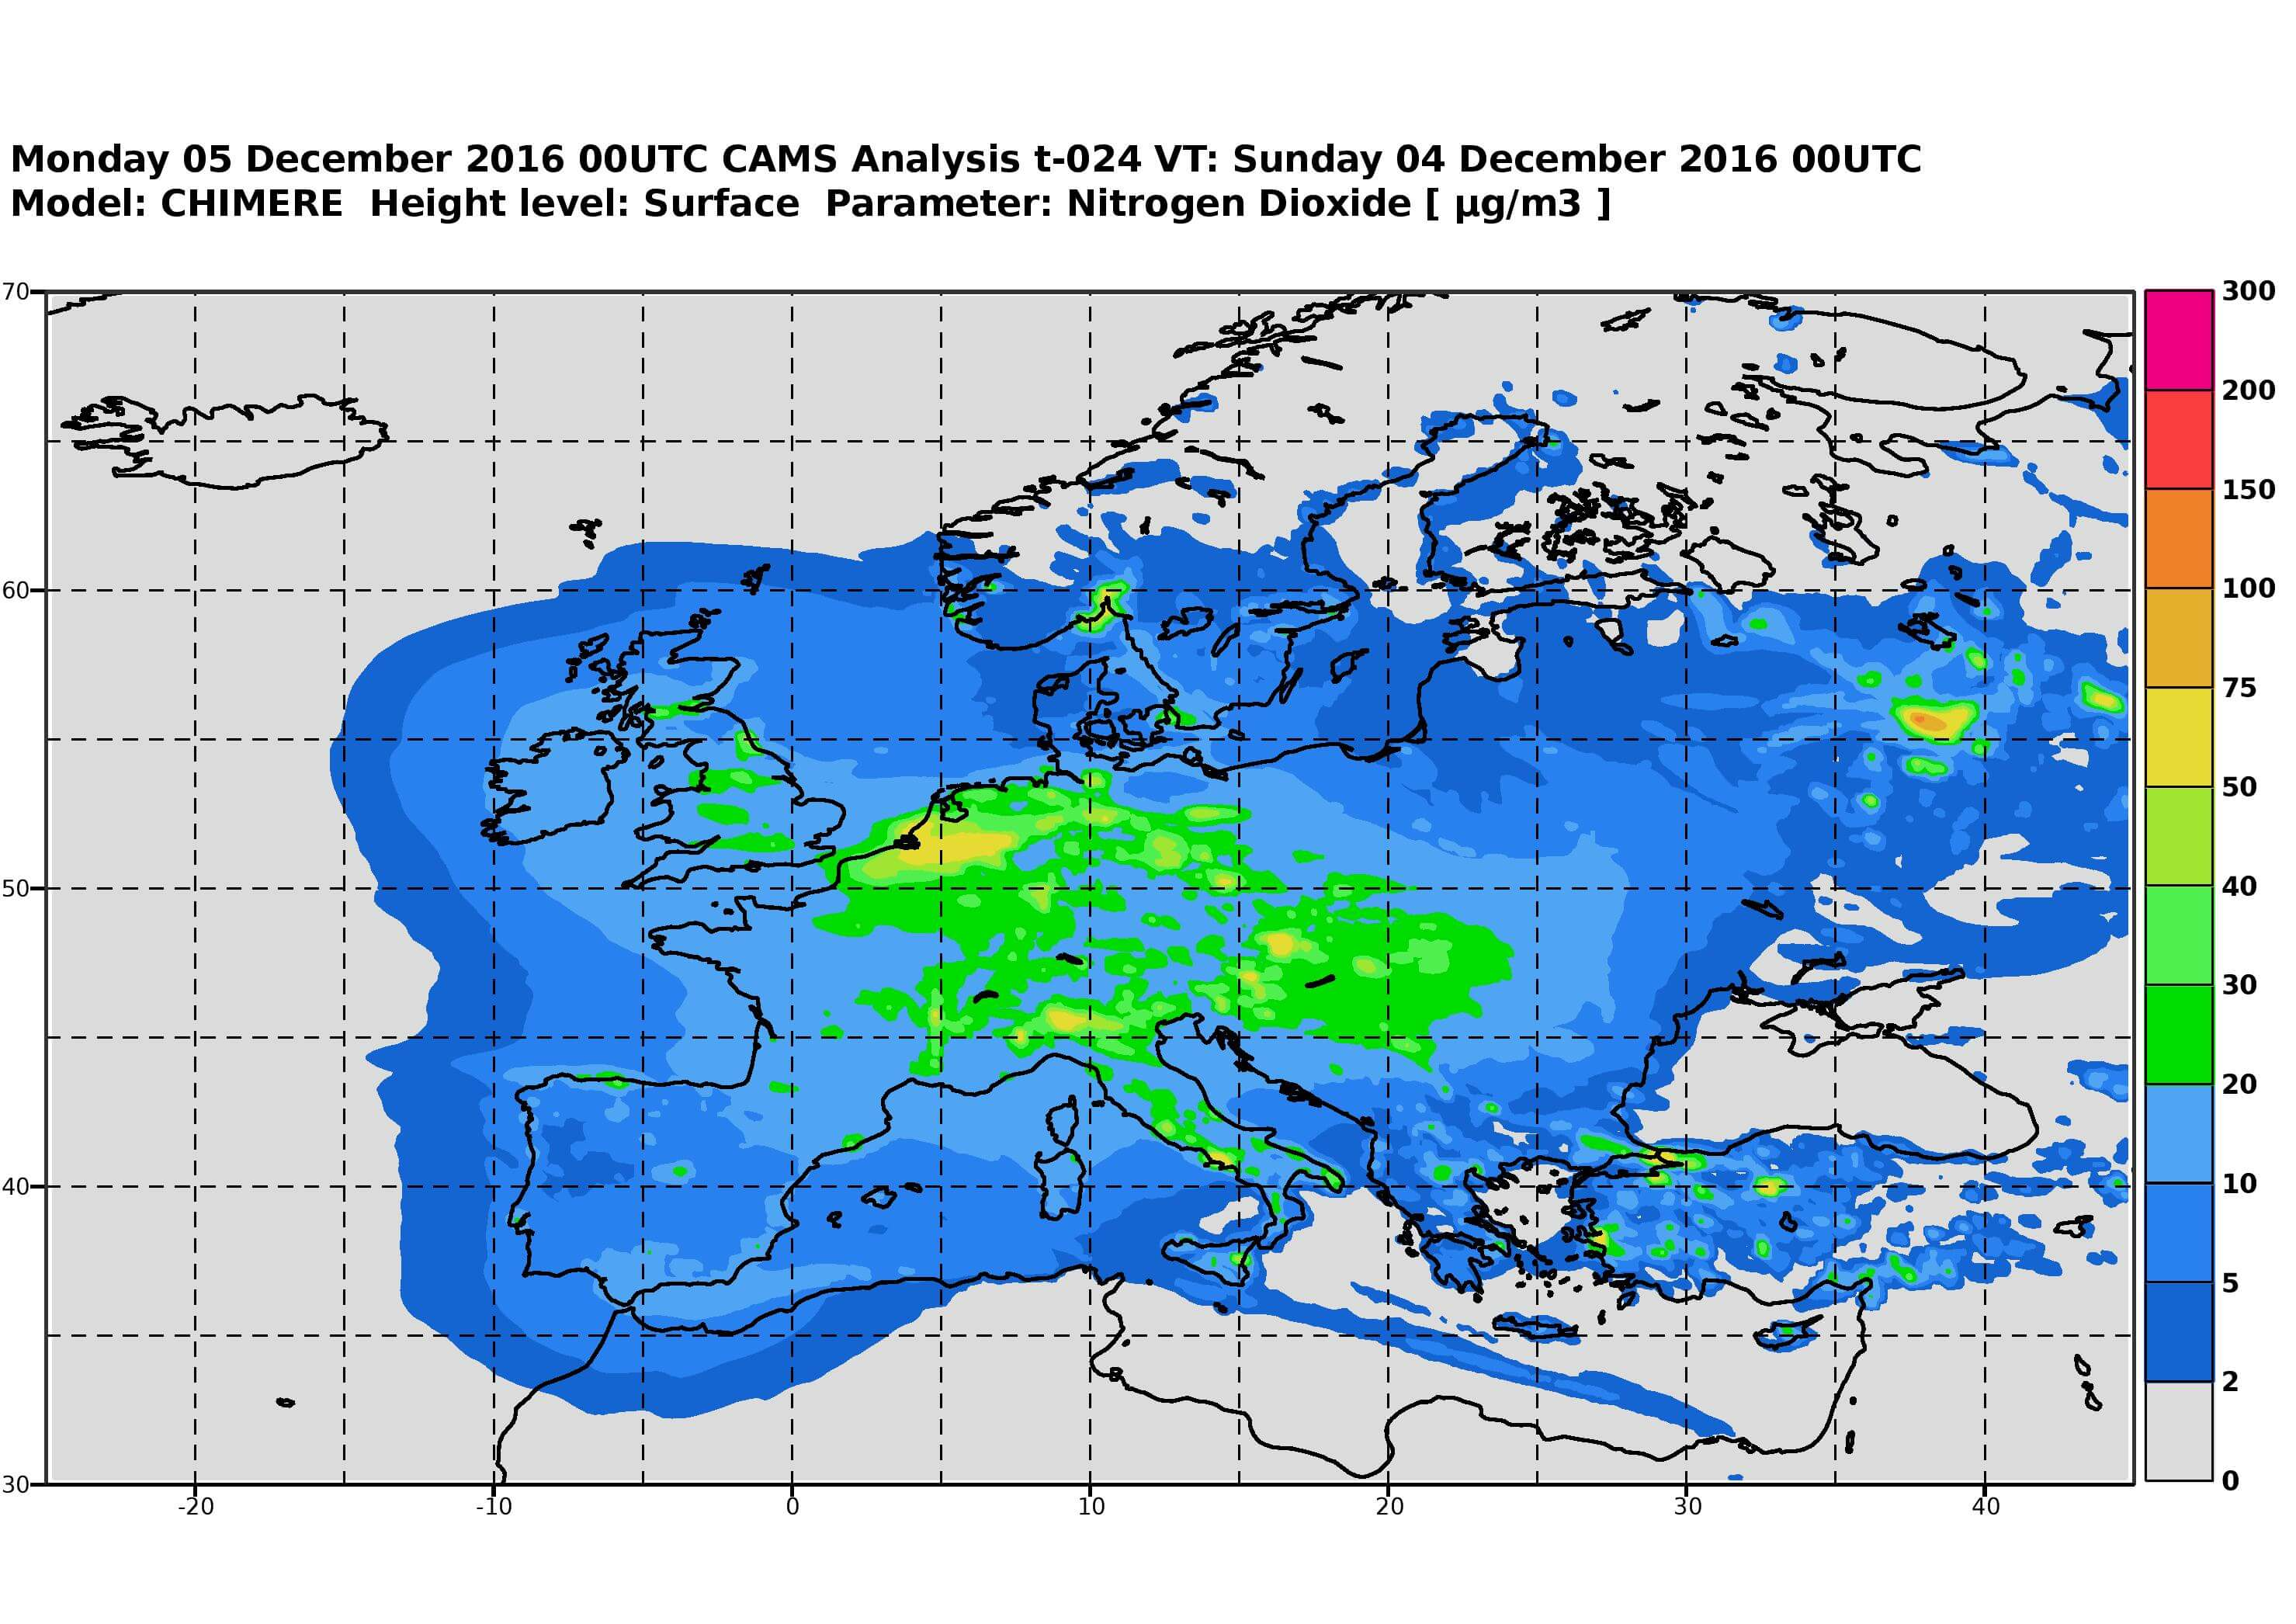
\includegraphics[keepaspectratio=true,width=\dimmin{}{\dimwidth{0.90}}]{images/chimere_analysis}{}\mdline{700}

%mdk-data-line={701}
\begin{mdbmargintb}{1ex}{}%mdk
\mdline{702}(b) \mdline{702} Analysis issued on December 5th, 2016%mdk
\end{mdbmargintb}%mdk%mdk
\end{mdblock}%mdk
\end{mdcolumn}%mdk
\\
\end{tabular}\end{mdtabular}
}
%mdk-data-line={703}
\mdhr{}%mdk

%mdk-data-line={704}
\noindent\mdline{704}\mdcaption{\textbf{Figure~\mdcaptionlabel{10}.}~\mdcaptiontext{Forecast and analysis maps of NO\mdsub{2} concentration for December 4th, 2016 issued by the CHIMERE model.}}%mdk
%mdk
\end{mdcenter}\label{chimere-map}%mdk
%mdk
\end{figure}%mdk

%mdk-data-line={709}
\noindent\mdline{709}Data files are very easy to download. Under the filters section there is a \mdline{709}\emph{Direct Data Access}\mdline{709} section with a checkbox for accepting the CAMS data licence.
Once the checkbox is checked we are presented with the details of the product (model, pollutant, base date/time) and an optional selectbox with available options depending on the product.
After an option is selected a direct download in NetCDF format is available by clicking the button.%mdk

%mdk-data-line={713}
\section{\mdline{713}5.\hspace*{0.5em}\mdline{713}Conclusions}\label{sec-conclusions}%mdk%mdk

%mdk-data-line={715}
\noindent\mdline{715}Satellites are capable of measuring the most important air pollutants, greenhouse gases and particles such as those from dust and pollen. They provide timely, spatially explicit, large-scale information on distribution in a cost-effective manner. When these data are coupled with ground-based measurements from monitoring stations and atmospheric chemistry models, accurate information on air quality can be provided in near-real time to support European air quality policies, air pollution mitigation and public health protection.%mdk

%mdk-data-line={717}
\mdline{717}CAMS provide services both global and regional, with each side having its advantages and drawbacks. For this reason, major updates are incorporated continually, new satellites are launched, and models used for prediction are also modified, in order to produce better assessments.%mdk

%mdk-data-line={719}
\mdline{719}When studying the usability of CAMS one must have in mind that it is essentially composed of two different services: global and regional.%mdk

%mdk-data-line={721}
\mdline{721}The global models C-IFS and IFS-LMD are much more mature and tested. However, the website of ECMWF that provides the results is not very functional and can be frustrating for the common user.%mdk

%mdk-data-line={723}
\mdline{723}On the other hand, the regional models are quite fresh and several were developed for a different purpose, however quarterly reports show that all models are constantly improving over time\mdline{723}\mdfootnote{13}{%mdk-data-line={727}
%mdk-data-line={727}
\noindent\mdline{727}https://atmosphere.copernicus.eu/documentation-regional-systems%mdk
\label{fn-reg-dossiers}%mdk%mdk
}\mdline{723}. Moreover, the website of regional services is very functional and easy to use, even by a completely inexperienced user.%mdk

%mdk-data-line={725}
\mdline{725}What anyone can conclude is that we are only at the beginning. CAMS is a very powerful and important service, which has enormous possibilities of continuous and large-scale monitoring with advanced satellite-based systems. Also, can provide timely and reliable long-term information for assessment and verification purposes. It is sure that with its predictions can contribute to EU efforts to monitor health-related environmental phenomena.%mdk

%mdk-data-line={729;out/final-report-bib.bbl.mdk:1}
%mdk-data-line={729;out/final-report-bib.bbl.mdk:2}
\mdsetrefname{References}%mdk
{\mdbibindent{0}%mdk
\begin{thebibliography}{32}%mdk
\label{sec-bibliography}%mdk

%mdk-data-line={./bibliography.bib:94}
\bibitem{annamalai2007combustion}Kalyan Annamalai. \emph{Combustion Science and Engineering}. CRC Press/Taylor \& Francis, Boca Raton. 2007.\label{annamalai2007combustion}%mdk%mdk

%mdk-data-line={./bibliography.bib:118}
\bibitem{beekmann2010modelling}M Beekmann, and R Vautard. \textquotedblleft{}A Modelling Study of Photochemical Regimes over Europe: Robustness and Variability.\textquotedblright{} \emph{Atmos. Chem. Phys} 10: 10067–10084. 2010.\label{beekmann2010modelling}%mdk%mdk

%mdk-data-line={./bibliography.bib:45}
\bibitem{bell2006exposure}Michelle L Bell, Roger D Peng, and Francesca Dominici. \textquotedblleft{}The Exposure-Response Curve for Ozone and Risk of Mortality and the Adequacy of Current Ozone Regulations.\textquotedblright{} \emph{Environmental Health Perspectives}. JSTOR, 532–536. 2006.\label{bell2006exposure}%mdk%mdk

%mdk-data-line={./bibliography.bib:342}
\bibitem{boucher2002history}O Boucher, and M Pham. \textquotedblleft{}History of Sulfate Aerosol Radiative Forcings.\textquotedblright{} \emph{Geophysical Research Letters} 29 (9). Wiley Online Library. 2002.\label{boucher2002history}%mdk%mdk

%mdk-data-line={./bibliography.bib:302}
\bibitem{bousserez2007evaluation}N Bousserez, JL Atti\'{e}, VH Peuch, M Michou, G Pfister, D Edwards, L Emmons, et al. \textquotedblleft{}Evaluation of the MOCAGE Chemistry Transport Model during the ICARTT/ITOP Experiment.\textquotedblright{} \emph{Journal of Geophysical Research: Atmospheres} 112 (D10). Wiley Online Library. 2007.\label{bousserez2007evaluation}%mdk%mdk

%mdk-data-line={./bibliography.bib:104}
\bibitem{epabulletin}Clean Air Technology Center, Information Transfer, Program Integration Division, Office of Air Quality Planning, Standards, U.S.~Environmental Protection Agency, and North Carolina Research Triangle Park. \emph{Nitrogen Oxides, Why and How They Are Controlled}. Nov. 1999.\label{epabulletin}%mdk%mdk

%mdk-data-line={./bibliography.bib:138}
\bibitem{colette2011air}Augustin Colette, Claire Granier, \O{}ivind Hodnebrog, Hermann Jakobs, Alberto Maurizi, Agnes Nyiri, Bertrand Bessagnet, et al. \textquotedblleft{}Air Quality Trends in Europe over the Past Decade: A First Multi-Model Assessment.\textquotedblright{} \emph{Atmospheric Chemistry and Physics} 11 (22). Copernicus GmbH: 11657–11678. 2011.\label{colette2011air}%mdk%mdk

%mdk-data-line={./bibliography.bib:259}
\bibitem{curier2012improving}RL Curier, R Timmermans, S Calabretta-Jongen, H Eskes, A Segers, D Swart, and M Schaap. \textquotedblleft{}Improving Ozone Forecasts over Europe by Synergistic Use of the LOTOS-EUROS Chemical Transport Model and in-Situ Measurements.\textquotedblright{} \emph{Atmospheric Environment} 60. Elsevier: 217–226. 2012.\label{curier2012improving}%mdk%mdk

%mdk-data-line={./bibliography.bib:1}
\bibitem{ebel2007advanced}Adolf Ebel, Michael Memmesheimer, Hermann J Jakobs, and Hendrik Feldmann. \textquotedblleft{}Advanced Air Pollution Models and Their Application to Risk and Impact Assessment.\textquotedblright{} In \emph{Air, Water and Soil Quality Modelling for Risk and Impact Assessment}, 83–92. Springer. 2007.\label{ebel2007advanced}%mdk%mdk

%mdk-data-line={./bibliography.bib:167}
\bibitem{fagerli2008trends}Hilde Fagerli, and Wenche Aas. \textquotedblleft{}Trends of Nitrogen in Air and Precipitation: Model Results and Observations at EMEP Sites in Europe, 1980\textendash{}2003.\textquotedblright{} \emph{Environmental Pollution} 154 (3). Elsevier: 448–461. 2008.\label{fagerli2008trends}%mdk%mdk

%mdk-data-line={./bibliography.bib:20}
\bibitem{forster2007changes}Piers Forster, Venkatachalam Ramaswamy, Paulo Artaxo, Terje Berntsen, Richard Betts, David W Fahey, James Haywood, et al. \textquotedblleft{}Changes in Atmospheric Constituents and in Radiative Forcing. Chapter 2.\textquotedblright{} In \emph{Climate Change 2007. The Physical Science Basis}. 2007.\label{forster2007changes}%mdk%mdk

%mdk-data-line={./bibliography.bib:54}
\bibitem{fowler2008ground}David Fowler, M Amann, F Anderson, M Ashmore, P Cox, M Depledge, D Derwent, et al. \textquotedblleft{}Ground-Level Ozone in the 21st Century: Future Trends, Impacts and Policy Implications.\textquotedblright{} \emph{Royal Society Science Policy Report} 15 (08). 2008.\label{fowler2008ground}%mdk%mdk

%mdk-data-line={./bibliography.bib:178}
\bibitem{genberg2013light}Johan Genberg, HAC Denier Van Der Gon, David Simpson, Erik Swietlicki, Hans Areskoug, David Beddows, Darius Ceburnis, et al. \textquotedblleft{}Light-Absorbing Carbon in Europe\textendash{}measurement and Modelling, with a Focus on Residential Wood Combustion Emissions.\textquotedblright{} \emph{Atmospheric Chemistry and Physics} 13 (17). Copernicus GmbH: 8719–8738. 2013.\label{genberg2013light}%mdk%mdk

%mdk-data-line={./bibliography.bib:160}
\bibitem{jonson2006first}J Jonson, P Wind, M Gauss, S Tsyro, A S\o{}vde, H Klein, I Isaksen, and L Tarras\'{o}n. \textquotedblleft{}First Results from the Hemispheric EMEP Model and Comparison with the Global Oslo CTM2 Model.\textquotedblright{} \emph{The Norwegian Meteorological Institute, Oslo, Norway}. 2006.\label{jonson2006first}%mdk%mdk

%mdk-data-line={./bibliography.bib:291}
\bibitem{josse2004radon}B Josse, P Simon, and V-H Peuch. \textquotedblleft{}Radon Global Simulations with the Multiscale Chemistry and Transport Model MOCAGE.\textquotedblright{} \emph{Tellus B} 56 (4). Wiley Online Library: 339–356. 2004.\label{josse2004radon}%mdk%mdk

%mdk-data-line={./bibliography.bib:312}
\bibitem{lacressonniere2014european}G Lacressonni\`{e}re, V-H Peuch, R Vautard, J Arteta, M D\'{e}qu\'{e}, M Joly, B Josse, V Mar\'{e}cal, and D Saint-Martin. \textquotedblleft{}European Air Quality in the 2030s and 2050s: Impacts of Global and Regional Emission Trends and of Climate Change.\textquotedblright{} \emph{Atmospheric Environment} 92. Elsevier: 348–358. 2014.\label{lacressonniere2014european}%mdk%mdk

%mdk-data-line={./bibliography.bib:280}
\bibitem{langner1998validation}Joakim Langner, Lennart Robertson, Christer Persson, and Anders Ullerstig. \textquotedblleft{}Validation of the Operational Emergency Response Model at the Swedish Meteorological and Hydrological Institute Using Data from ETEX and the Chernobyl Accident.\textquotedblright{} \emph{Atmospheric Environment} 32 (24). Elsevier: 4325–4333. 1998.\label{langner1998validation}%mdk%mdk

%mdk-data-line={./bibliography.bib:10}
\bibitem{menut2010atmospheric}Laurent Menut, and Bertrand Bessagnet. \textquotedblleft{}Atmospheric Composition Forecasting in Europe.\textquotedblright{} In \emph{Annales Geophysicae}, 28:61–74. 1. 2010.\label{menut2010atmospheric}%mdk%mdk

%mdk-data-line={./bibliography.bib:111}
\bibitem{menut2013chimere}L Menut, B Bessagnet, D Khvorostyanov, M Beekmann, N Blond, A Colette, I Coll, et al. \textquotedblleft{}CHIMERE 2013: A Model for Regional Atmospheric Composition Modelling, Geosci. Model Dev., 6, 981\textendash{}1028, Doi: 10.5194.\textquotedblright{} gmd-6-981-2013. 2013.\label{menut2013chimere}%mdk%mdk

%mdk-data-line={./bibliography.bib:74}
\bibitem{mollenhauer2010handbook}Klaus Mollenhauer, and Helmut Tschöke. \emph{Handbook of Diesel Engines}. Springer. 2010.\label{mollenhauer2010handbook}%mdk%mdk

%mdk-data-line={./bibliography.bib:219}
\bibitem{monteiro2013bias}A Monteiro, I Ribeiro, O Tchepel, E S\'{a}, J Ferreira, A Carvalho, V Martins, et al. \textquotedblleft{}Bias Correction Techniques to Improve Air Quality Ensemble Predictions: Focus on O3 and PM over Portugal.\textquotedblright{} \emph{Environmental Modeling \& Assessment} 18 (5). Springer: 533–546. 2013.\label{monteiro2013bias}%mdk%mdk

%mdk-data-line={./bibliography.bib:82}
\bibitem{omidvarborna2015113}Hamid Omidvarborna, Ashok Kumar, and Dong-Shik Kim. \textquotedblleft{}NOx Emissions from Low-Temperature Combustion of Biodiesel Made of Various Feedstocks and Blends.\textquotedblright{} \emph{Fuel Processing Technology} 140: 113–118. 2015. doi:\href{https://dx.doi.org/10.1016/j.fuproc.2015.08.031}{10.1016/j.fuproc.2015.08.031}.\label{omidvarborna2015113}%mdk%mdk

%mdk-data-line={./bibliography.bib:230}
\bibitem{paschalidi2015inverse}Zoi Paschalidi. \textquotedblleft{}Inverse Modelling for the Tropospheric Chemical State Estimation by 4-Dimensional Variational Data Assimilation from Routinely and Campaign Platforms.\textquotedblright{} Phdthesis, Universit\"{a}t zu K\"{o}ln. 2015.\label{paschalidi2015inverse}%mdk%mdk

%mdk-data-line={./bibliography.bib:352}
\bibitem{reddy2005aerosol}M Shekar Reddy, Olivier Boucher, Yves Balkanski, and Michael Schulz. \textquotedblleft{}Aerosol Optical Depths and Direct Radiative Perturbations by Species and Source Type.\textquotedblright{} \emph{Geophysical Research Letters} 32 (12). Wiley Online Library. 2005.\label{reddy2005aerosol}%mdk%mdk

%mdk-data-line={./bibliography.bib:322}
\bibitem{rouil2009prev}Laurence Rouil, C\'{e}cile Honore, Robert Vautard, Matthias Beekmann, Bertrand Bessagnet, Laure Malherbe, Fr\'{e}d\'{e}rik Meleux, et al. \textquotedblleft{}PREV’AIR.\textquotedblright{} \emph{Bulletin of the American Meteorological Society} 90 (1). American Meteorological Society: 73. 2009.\label{rouil2009prev}%mdk%mdk

%mdk-data-line={./bibliography.bib:27}
\bibitem{sabziparvar1998changes}Ali A Sabziparvar, De F Forster, and Keith P Shine. \textquotedblleft{}Changes in Ultraviolet Radiation due to Stratospheric and Tropospheric Ozone Changes since Preindustrial Times.\textquotedblright{} \emph{Journal of Geophysical Research} 103 (D20): 26107–26113. 1998.\label{sabziparvar1998changes}%mdk%mdk

%mdk-data-line={./bibliography.bib:237}
\bibitem{schaap2008lotos}Martijn Schaap, Renske MA Timmermans, Michiel Roemer, GAC Boersen, Peter Builtjes, Ferd Sauter, Guus Velders, and Jeanette Beck. \textquotedblleft{}The LOTOS-EUROS Model: Description, Validation and Latest Developments.\textquotedblright{} \emph{International Journal of Environment and Pollution} 32 (2). Inderscience Publishers: 270–290. 2008.\label{schaap2008lotos}%mdk%mdk

%mdk-data-line={./bibliography.bib:37}
\bibitem{seinfeld2006atmospheric}John H Seinfeld, and Spyros N Pandis. \emph{Atmospheric Chemistry and Physics. Hoboken}. Volume 450. NJ: Wiley. 2006.\label{seinfeld2006atmospheric}%mdk%mdk

%mdk-data-line={./bibliography.bib:63}
\bibitem{sitch2007indirect}S Sitch, PM Cox, WJ Collins, and C Huntingford. \textquotedblleft{}Indirect Radiative Forcing of Climate Change through Ozone Effects on the Land-Carbon Sink.\textquotedblright{} \emph{Nature} 448 (7155). Nature Publishing Group: 791–794. 2007.\label{sitch2007indirect}%mdk%mdk

%mdk-data-line={./bibliography.bib:333}
\bibitem{sofiev2008construction}Mikhail Sofiev, Michael Galperin, and Eugene Genikhovich. \textquotedblleft{}A Construction and Evaluation of Eulerian Dynamic Core for the Air Quality and Emergency Modelling System SILAM.\textquotedblright{} In \emph{Air Pollution Modeling and Its Application XIX}, 699–701. Springer. 2008.\label{sofiev2008construction}%mdk%mdk

%mdk-data-line={./bibliography.bib:269}
\bibitem{vlemmix2015max}T Vlemmix, HJ Eskes, AJM Piters, M Schaap, FJ Sauter, H Kelder, and PF Levelt. \textquotedblleft{}MAX-DOAS Tropospheric Nitrogen Dioxide Column Measurements Compared with the Lotos-Euros Air Quality Model.\textquotedblright{} \emph{Atmospheric Chemistry and Physics} 15 (3). Copernicus GmbH: 1313–1330. 2015.\label{vlemmix2015max}%mdk%mdk

%mdk-data-line={./bibliography.bib:248}
\bibitem{de2011six}Martijn de Ruyter de Wildt, Henk Eskes, Astrid Manders, Ferd Sauter, Martijn Schaap, Daan Swart, and Peter van Velthoven. \textquotedblleft{}Six-Day PM 10 Air Quality Forecasts for the Netherlands with the Chemistry Transport Model Lotos-Euros.\textquotedblright{} \emph{Atmospheric Environment} 45 (31). Elsevier: 5586–5594. 2011.\label{de2011six}%mdk%mdk
\par%mdk
\end{thebibliography}}%mdk%mdk%mdk


\end{document}
